%%%%%%%%%%%%%%%%%%%%%%%%%%%%%%%%%%%%%%%%%%%%%%%%%%%%%%%%%%%%%%%%%%%%%%%%%%%
%
% Generic template for TFC/TFM/TFG/Tesis
%
% $Id: introduccion.tex,v 1.19 2015/02/24 23:21:54 macias Exp $
%
% By:
%  + Javier Macías-Guarasa. 
%    Departamento de Electrónica
%    Universidad de Alcalá
%  + Roberto Barra-Chicote. 
%    Departamento de Ingeniería Electrónica
%    Universidad Politécnica de Madrid   
% 
% Based on original sources by Roberto Barra, Manuel Ocaña, Jesús Nuevo,
% Pedro Revenga, Fernando Herránz and Noelia Hernández. Thanks a lot to
% all of them, and to the many anonymous contributors found (thanks to
% google) that provided help in setting all this up.
%
% See also the additionalContributors.txt file to check the name of
% additional contributors to this work.
%
% If you think you can add pieces of relevant/useful examples,
% improvements, please contact us at (macias@depeca.uah.es)
%
% Copyleft 2013
%
%%%%%%%%%%%%%%%%%%%%%%%%%%%%%%%%%%%%%%%%%%%%%%%%%%%%%%%%%%%%%%%%%%%%%%%%%%%

\chapter{Empirical Work}\label{chp:empwork}

In this chapter, we cover the experimental work carried out. Firstly, we 
describe the datasets used for the experimentation; then, the supervised 
classifiers evaluated; the evaluation metrics chosen; and finally, present and 
discuss the results.

%%%%%%%%%%%%%%%%%%%%%%%%%%%%%%%%%%%%%%%%%%%%%%%%%%%%%%%%%%%%%%%%%%%%%%%%%%%%%%%%
\section{Datasets}\label{sec:datasets}

In this work, publicly available datasets in the domain of Software defect 
prediction were used, were used, the Jureczko and Madeyski dataset
\footnote{\url{http://snow.iiar.pwr.wroc.pl:8080/MetricsRepo/}} 
\cite{Jureczko2010, MadeyskiJ2015}, the Apache dataset 
(\cite{Zimmermann07Eclipse}) and the Harman Search Base dataset 
\cite{Harman2014ssbse}. 

From the first cluster of datasets, 15 open source projects are the ones chosen 
(a total of 8 are used for this project). The number of defects found in each 
class collected from the Software Management System (SCM) using a regular 
expression. The datasets are publicly available  (can be found in the PROMISE 
repository~\cite{promiserepo}). These datasets have been used in previous 
researches, \cite{Xu2018, Wang2016, Xia2016}, which allows comparing and 
analyzing the obtained results.

A sample can be considered as \textit{defective} when the number of defects 
inside the class is more than 0. Similarly, if the number of defects is 0, then 
the class is \textit{non-defective}. This allows a binary classification, making 
easier handling results, operations and comparisons.

\begin{center}
\begin{longtable}{ | l | l | }
\caption{Defect Metrics Dataset Variables}\label{tab:dataJureczkoMetrics} \\

\hline
 \emph{Metric} & \emph{Description} \\
\hline 
\hline
\endfirsthead
\multicolumn{2}{c}{\tablename\ \thetable\ -- \textit{Continued from previous page}} \\
\hline
\emph{Metric} & \emph{Description} \\
\hline 
\hline
\endhead
\hline
\multicolumn{2}{r}{\textit{Continued on next page}}
\endfoot
\hline
\endlastfoot
WMC    &    Weighted methods per class \cite{Chidamber1994} \\
DIT    &    Depth of Inheritance Tree \cite{Chidamber1994} \\
NOC    &    Number of Children \cite{Chidamber1994} \\
CBO    &    Coupling between object classes \cite{Chidamber1994} \\
RFC    &    Response for a Class \cite{Chidamber1994} \\
LCOM   &    Lack of cohesion in methods \cite{Chidamber1994} \\
Ca     &    Afferent couplings \cite{Martin1994} \\
Ce     &    Efferent couplings \cite{Martin1994} \\
NPM    &    Number of Public Methods \cite{Bansiya2002} \\
LCOM3  &    Lack of cohesion in methods \cite{Henderson-Sellers1995} \\
LOC    &    Lines of Code \cite{Bansiya2002} \\
DAM    &    Data Access Metric \cite{Bansiya2002} \\
MOA    &    Measure of Aggregation \cite{Bansiya2002} \\
MFA    &    Measure of Functional Abstraction \cite{Bansiya2002} \\
CAM    &    Cohesion Among Methods of Class \cite{Bansiya2002} \\
IC     &    Inheritance Coupling \cite{Tang} \\
CBM    &    Coupling Between Methods \cite{Tang} \\
AMC    &    Average Method Complexity \cite{Tang} \\
MAX\textunderscore CC    &    Maximum McCabe's cyclomatic complexity \cite{McCabe1976} \\
AVG\textunderscore CC    &    Average McCabe's cyclomatic complexity \cite{McCabe1976} \\
\hline
\end{longtable}
\end{center}

There is another sole dataset obtained from the same source as the previous 
collection of datasets, with a very similar structure of data, the 
\textit{Apache} dataset. It has the same origin and objective as its 
predecessors.

On the second cluster of datasets, the data comes from a total of 8 different 
Hadoop versions. Their original purpose is to train a search based fault 
prediction system. 

Similarly to Jureczko and Madeyski dataset \cite{Jureczko2010, MadeyskiJ2015}, 
it uses: (1) WMC, (2) DIT, (3), NOC, (4) CBO, (5) RFC, (6) LCOM, (7) NOM, and 
(8) LOC; metrics to define each dataset.

Regarding more information on the content of the datasets the next table (see 
Table~\ref{tab:metrics-description}) summarizes the number of samples on each 
dataset and further valuable information, such as the absolute and relative 
number of defects for those datasets.

\begin{center}
\begin{longtable}{ | c | c | c c c c | }
\caption{Description of the Datasets} \label{tab:metrics-description} \\

\hline
\emph{Project} & \emph{Version} & 
\emph{\#instances} & \emph{\#Non-Defective} & \emph{\#Defective} & \emph{\%Defective} \\
\hline 
\hline
\endfirsthead
\multicolumn{6}{c}{\tablename\ \thetable\ -- \textit{Continued from previous page}} \\
\hline
\emph{Project} & \emph{Version} & 
\emph{\#instances} & \emph{\#Non-Def} & \emph{\#Def} & \emph{\%Def} \\
\hline
\hline
\endhead
\hline
\multicolumn{6}{r}{\textit{Continued on next page}}
\endfoot
\hline
\endlastfoot

\multirow{5}{*}{ant} &  
    1.3 &   125 &   105 &    20 &   16.00 \\
&   1.4 &   178 &   138 &    40 &   22.47 \\ 
&   1.5 &   293 &   261 &    32 &   10.92 \\
&   1.6 &   351 &   259 &    92 &   26.21 \\
&   1.7 &   745 &   579 &   166 &   22.28 \\

\hline
\multirow{1}{*}{apache} &  
    -   &   191 &   107 &   84  &   43.98 \\

\hline
\multirow{4}{*}{camel} &   
    1.0 &   339 &   326 &    13 &    3.83 \\
&   1.2 &   608 &   392 &   216 &   35.52 \\
&   1.4 &   872 &   727 &   145 &   16.62 \\
&   1.6 &   965 &   777 &   188 &   19.48 \\

\hline
\multirow{8}{*}{hadoop} &
    0.1 &   141 &    91 &    50 &   35.60 \\
&   0.2 &   191 &   149 &    42 &   21.99 \\
&   0.3 &   211 &   158 &    53 &   25.12 \\
&   0.4 &   201 &   159 &    42 &   20.90 \\
&   0.5 &   217 &   180 &    37 &   17.05 \\
&   0.6 &   234 &   203 &    31 &   13.25 \\
&   0.7 &   250 &   202 &    48 &   19.20 \\
&   0.8 &   240 &   224 &    16 &    6.67 \\

\hline
\multirow{2}{*}{ivy} &   
    1.4 &   241 &   225 &    16 &    6.63 \\
&   2.0 &   352 &   312 &    40 &   11.36 \\

\hline
\multirow{5}{*}{jedit} & 
    3.2 &   272 &   182 &    90 &   33.08 \\
&   4.0 &   306 &   231 &    75 &   24.50 \\
&   4.1 &   312 &   233 &    79 &   25.32 \\
&   4.2 &   367 &   319 &    48 &   13.07 \\
&   4.3 &   492 &   481 &    11 &    2.23 \\

\hline
\multirow{3}{*}{log4j} & 
    1.0 &   135 &   101 &    34 &   25.18 \\
&   1.1 &   109 &    72 &    37 &   33.94 \\
&   1.2 &   205 &    16 &   189 &   92.19 \\

\hline
\multirow{3}{*}{synapse} &
    1.0 &   157 &   141 &    16 &   10.19 \\
&   1.1 &   222 &   162 &    60 &   27.02 \\
&   1.2 &   256 &   170 &    86 &   33.59 \\

\hline
\multirow{4}{*}{xalan} & 
    2.4 &   723 &   613 &   110 &   15.21 \\
&   2.5 &   803 &   416 &   387 &   48.19 \\
&   2.6 &   885 &   474 &   411 &   46.44 \\
&   2.7 &   909 &    11 &   898 &   98.78 \\

\hline
\multirow{3}{*}{xerces} &
    1.2 &   440 &   369 &    71 &   16.13 \\
&   1.3 &   453 &   384 &    69 &   15.23 \\
&   1.4 &   588 &   151 &   437 &   74.31 \\
\hline

\end{longtable}
\end{center}

The experiments of this paper use the latest version of the datasets 
\textit{ant}, \textit{apache}, \textit{camel}, \textit{hadoop}, \textit{ivy},
\textit{jedit}, \textit{log4j}, \textit{xalan} and \textit{xerces}; alongide
all the available versions of the \textit{hadoop} dataset.

%%%%%%%%%%%%%%%%%%%%%%%%%%%%%%%%%%%%%%%%%%%%%%%%%%%%%%%%%%%%%%%%%%%%%%%%%%%%%%%%
\section{Supervised Classifiers}

This work makes use of several supervised learning algorithms. The 
experiments carried out use the following algorithms:

\begin{description}
    \item [Naive Bayes] (NB)~\cite{Mit97} is a classifier that works on 
	conditional probabilities, uses the Bayes theorem to predict the class for 
	each data input. Calculates the probability of a certain event, given prior 
	knowledge. This classifier assigns a set of attributes $a_{1}, \ldots, 
	a_{n}$ to a given class $C$ so that the probability of the class description 
	value of the attributes instances is maximal: $P(C|a_{1}, \ldots, a_n)$. The 
	probability of the hypothesis, given that the evidence is true, is the 
	probability of the evidence, given the hypothesis is true, multiplied by the 
	probability of the hypothesis; in relation to the probability of the 
	evidence. See Eq.~\ref{eq:bayes}.
    
    \begin{equation}\label{eq:bayes}
        P(H|E) = \frac{(E|H) * P(H)}{P(E)}
    \end{equation}
    
    For this project it has been selected the Gaussian Naive Bayes from 
	\texttt{scikit-learn}
	\footnote{\url{https://scikit-learn.org/stable/modules/generated/sklearn.naive_bayes.GaussianNB.html}} 
	to perform the experimentation. Being \textit{Gaussian} means that the 
	likelihood of the features is assumed to be Gaussian. The formula is given 
	by Eq.~\ref{eq:gaussian}.
    
    \begin{equation}\label{eq:gaussian}
        P(x_{i}|y)=(\frac{1}{\sqrt{2\pi \sigma^{2}_{y}}})\exp{(-\frac{(x_{i} - \mu _{y})^2}{2\sigma^{2}_{y}})}
    \end{equation}
    
    \item [Decision Trees] can be seen as rules with a root node, branches are 
	conditions and leaves correspond to classes. There are many decision trees 
	algorithm such as CART (Classification And Regression 
	Trees)~\cite{Breiman1984} is a non-parametric decision tree, similar to 
	\textbf{C4.5}~\cite{Quinlan1993}. 

	CART constructs a two branch bifurcation of the most discriminating 
	attribute, based on the Gini index. It can generate either classification or 
	regression trees - depends on the variable (categorical or numeric, 
	respectively). The implementation available in 
	\texttt{scikit-learn}~\cite{scikit-learn}
	\footnote{\url{https://scikit-learn.org/stable/modules/tree.html}} is an 
	optimised version of this algorithm, although it does not support 
	categorical variables.
    
    \item [Nearest Centroid] classifier\cite{conformal2014},  \textbf{Nearest 
	Prototype} classifier, or \textbf{Rocchio classifier} for its similarity to 
	an algorithm with the same name (see Eq.\ref{eq:rocchio}). 
    
    \begin{equation}\label{eq:rocchio}
        \overrightarrow{Q_{m}} =  (a \cdot \overrightarrow{Q_{o}}) + (b \cdot 
        \frac{1}{\lvert D_{r} \rvert} \cdot \sum_{\overrightarrow{D_{j}} \in 
        D_{r}} \overrightarrow{D_{j}}) - (c \cdot \frac{1}{\lvert D_{nr} 
        \rvert} \cdot \sum_{\overrightarrow{D_{k}} \in D_{nr}} 
        \overrightarrow{D_{k}})
    \end{equation}
    
    The labels of a given sample are assigned by evaluating the classes of 
	training samples whose mean is closest to the evaluated point. The training 
	procedure, given a labeled training set ${(\overrightarrow{x_{1}}, y_{1}), 
	\ldots,  (\overrightarrow{x_{n}}, y_{n})}$ with class labels $y_{i} \in Y$, 
	compute the per-class centroid with Eq.~\ref{eq:knntrain}.
    
    \begin{equation}\label{eq:knntrain}
        \overrightarrow{\mu _{l}} = \frac{1}{\lvert C_{l} \rvert} \sum_{i \in 
        C_{l}} \overrightarrow{x_{i}}
    \end{equation}
    
    \noindent where $C_{l}$ is the set of indices of samples belonging to class 
	$l \in Y$.  The prediction functions, takes the class assigned to an 
	observation $\overrightarrow{x}$ is Eq.~\ref{eq:knnpred}.
    
    \begin{equation}\label{eq:knnpred}
        \overrightarrow{y} = argmin_{l \in Y} \lvert\lvert \overrightarrow{\mu _{l}} - \overrightarrow{x} \rvert\rvert
    \end{equation}

\end{description}

%%%%%%%%%%%%%%%%%%%%%%%%%%%%%%%%%%%%%%%%%%%%%%%%%%%%%%%%%%%%%%%%%%%%%%%%%%%%%%%%
\section{Evaluation Metrics}\label{sec:ev-metrics}

Part of the process of applying a classification algorithm is to measure the 
success and the results of the training. In order to do it, some metrics can be 
calculated out of the testing to the trained classifier. Here is where the
Confusion Matrix comes at hand. The Confusion Matrix (see 
Table~\ref{tab:conf-matrix}) allows us to summarize the performance of a given 
classification algorithm, it is also the foundation of many of the performance 
metrics used in classification by:

% --> Confusion Matrix
\begin{table}[h!]
\centering
\footnotesize
\caption{Confusion Matrix for Binary Classification}
\label{tab:conf-matrix}
\begin{tabular}{c c | p{2.5cm} | p{2.5cm} }
% ROW1
  & & \multicolumn{2}{c}{\emph{Actual Class}}\\
% ROW2
  & &    \emph{Positive} & \emph{Negative} \\
% ROW3
  \hline
  \multirow{4}{*}{\emph{Predicted Class}}
  &\emph{Positive} & True Positive \newline ($TP$) & False Positive \newline ($FP$)\\
% ROW 4
  %\hline
  \cline{2-4}
  &\emph{Negative} & False Negative \newline ($FN$) & True Negative\newline ($TN$)\\
\end{tabular}
\end{table}

\begin{description}
 \item [True Positive (TP)] - Data is correctly classified as positive.
 \item [True Negative (TN)] - Data is correctly classified as negative.
 \item [False Positive (FP)] - Data being negative classified as positive.
 \item [False Negative (FN)] - Data being positive classified as negative. 
\end{description} 

These specifications indicate that the input data should have a binary target: 
one value that can be classified as \textit{positive} and a second value that 
can be classified as negative. From this statistical classification
\footnote{Also know as error matrix.}, many performance measures can be 
calculated. Some of the most widely used metrics, and the ones used in this 
paper are explained next.

%%%%%%%%%%%%%%%%%%%%%%%%%%%%%%%%%%%%%%%%%%%%%%%%%%%%%%%%%%%%%%%%%%%%%%
\subsection{Precision}    
 
Also know as Positive Predictive Value (PPV). It is the relation 
between the \textit{true positives} calculated and the overall positives 
detected by the classification algorithm (see Eq.~\ref{eq:ppv}).
 
\begin{equation}\label{eq:ppv}
    PPV = \frac{TP}{TP + FP} = 1 - FDR
\end{equation}

%%%%%%%%%%%%%%%%%%%%%%%%%%%%%%%%%%%%%%%%%%%%%%%%%%%%%%%%%%%%%%%%%%%%%%
\subsection{Recall} 

Also known as sensitivity, hit rate, or True Positive 
Rate (TPR). It stands for the relation between the \textit{true positives} 
calculated and the real number of positives (see Eq.~\ref{eq:tpr}).

\begin{equation}\label{eq:tpr}
    TPR = \frac{TP}{P} = \frac{TP}{TP + FN} = 1 - FNR
\end{equation}

%%%%%%%%%%%%%%%%%%%%%%%%%%%%%%%%%%%%%%%%%%%%%%%%%%%%%%%%%%%%%%%%%%%%%%
\subsection{Fall-out}

Also called False Positive Rate (FPR). It is the probability of rejecting 
(falsely) the null hypothesis\footnote{General statement or default position
that there is no relationship between two measured phenomena or no
association among groups.} for a particular test (see Eq.~\ref{eq:fpr}).

\begin{equation}\label{eq:fpr}
    FPR = \frac{FP}{N} = \frac{FP}{FP + TN} = 1 - TNR
\end{equation}
    
%%%%%%%%%%%%%%%%%%%%%%%%%%%%%%%%%%%%%%%%%%%%%%%%%%%%%%%%%%%%%%%%%%%%%%
\subsection{Balance Accuracy}

It goes by the acronym BA. It is a metric generally used to evaluate how
good is a (binary) classifier. It is a measure that comes in specially 
handy for imbalanced datasets. Its formula is represented by the mean of
\textit{sensitivity} and \textit{specificity} (see Eq.~\ref{eq:ba}).

\begin{equation}\label{eq:ba}
    BA = \frac{TPR + TNR}{2}
\end{equation}
    
%%%%%%%%%%%%%%%%%%%%%%%%%%%%%%%%%%%%%%%%%%%%%%%%%%%%%%%%%%%%%%%%%%%%%%
\subsection{F-Measure} 
 
Also known as $F_1$, or \textit{S\o rensen-Dice coefficient} (independently 
developed by S\o rensen~\cite{sorensen1948} and Dice~\cite{dice1945}) is the 
harmonic mean of precision and sensitivity, the two previous measures, which 
measures accuracy (see Eq.~\ref{eq:f1}). It is twice the relation of the 
multiplication between \textit{recall} and \textit{precision} and their 
addition. It is commonly used in highly imbalanced datasets but there are also 
some criticisms as it does not take into account the \textit{True Negative} 
(\textit{TN}) cases.

\begin{equation}\label{eq:f1}
    F_1 = 2 \cdot \frac{PPV \cdot TPR}{PPV + TPR} = \frac{2 \cdot TP}{2 \cdot TP + FP + FN}
\end{equation}
    
%%%%%%%%%%%%%%%%%%%%%%%%%%%%%%%%%%%%%%%%%%%%%%%%%%%%%%%%%%%%%%%%%%%%%%    
\subsection{MCC} 

The Matthews Correlation Coefficient (MCC)~\cite{Matthews1975} or \textit{phi} 
coefficient measures the quality of a binary classification robust to the 
imbalance problem (Eq.~\ref{eq:mcc}). Its range values are between -1 and +1, 
where -1 represents complete inconsistency (disagreement), 0 indicates that the 
prediction is no better than a random prediction; and +1 would be a perfect 
prediction.  

\begin{equation}\label{eq:mcc}
    MCC = \frac{TP \cdot TN - FP \cdot FN}{\sqrt{(TP + FP)(TP + FN)(TN + FP)(TN + FN)}}
\end{equation}

%%%%%%%%%%%%%%%%%%%%%%%%%%%%%%%%%%%%%%%%%%%%%%%%%%%%%%%%%%%%%%%%%%%%%%
\subsection{Receiver Operating Characteristic Curve}\label{sec:roc}

The Receiver Operating Characteristic (ROC)\cite{Fawcett2006} Curve represents 
graphically the True Positive Rate (TPR) versus the False Positive Rate (FPR) as 
shown in Figure~\ref{fig:roc}.

\begin{figure}
\centering
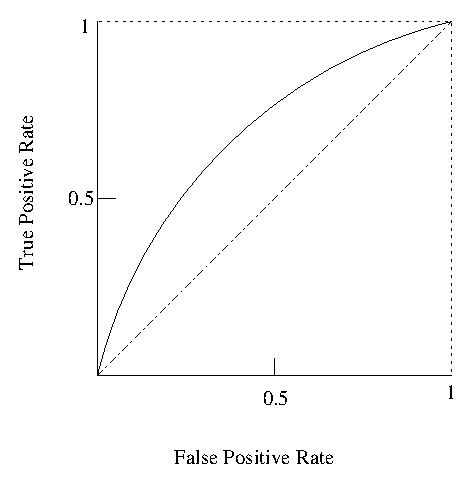
\includegraphics[width=.4\textwidth]{roc} % width=9cm, height=6cm
\caption{ROC Curve}
\label{fig:roc}
\end{figure}

Once the curve is plotted, the more the curve gets similar to a slope of 
$TPR = FPR$ the more imbalance that can be found in the dataset. It provides
graphical visualization of the results. 

The Area Under the ROC Curve (AUC) is a quality measure between positive and 
negative rates with a single value. This metric allows to compare models.

An approximation to the function can be calculated with Eq~\ref{eq:auc}.

\begin{equation}\label{eq:auc}
    AUC = \frac{1 + TP_{r} - FP_{r}}{2}
\end{equation}


Typically, three unbiased metrics, i.e., AUC, F-score 
(\cite{sorensen1948,dice1945}), Matthews Correlation Coefficient 
(MCC - \cite{Matthews1975}), are used to evaluate the performance on imbalanced 
datasets. Other measures cannot be used when data is highly imbalanced, like 
\textit{accuracy} (\textit{Acc}) (defined by Eq.~\ref{eq:accuracy}), as it does 
not take into account the number of labels of different classes.

\begin{equation}\label{eq:accuracy}
    Acc = \frac{TP + TN}{TP + TN + FP + FN}
\end{equation}

%%%%%%%%%%%%%%%%%%%%%%%%%%%%%%%%%%%%%%%%%%%%%%%%%%%%%%%%%%%%%%%%%%%%%%%%%%%%%%%%
\section{Results and discussion}\label{sec:results}

%%%%%%%%%%%%%%%%%%%%%%%%%%%%%%%%%%%%%%%%%%%%%%%%%%%%%%%%%%%%%%%%%%%%%%

\subsection{Methodology}

To answer the research questions stated in Section \ref{sec:aim-obj}, we run 
several experiments. First, we analyse the complexity metrics (see 
Section~\ref{sec:ecol}) from all selected datasets (see 
Section~\ref{sec:datasets}). Then, we retrieve some analytical metrics (see 
Section~\ref{sec:ev-metrics}), applying $K$-fold Cross
Validation to those datasets. Finally, we repeat the process applying some 
under/oversampling techniques with $K$-CV (see 
Sections~\ref{sec:undersampling} and~\ref{sec:oversampling}, respectively).

As the final aim is to see how complexity metrics affect classification and 
therefore the analytical metrics, a final section is going to summarize the 
results obtained and the conclusions drawn out of those measures and answer the 
research questions.

%%%%%%%%%%%%%%%%%%%%%%%%%%%%%%%%%%%%%%%%%%%%%%%%%%%%%%%%%%%%%%%%%%%%%%
\subsection{Data Complexity Metrics Analysis}

As it has been mentioned in \textit{Data Complexity Metrics} (see 
Section ~\ref{sec:ecol}), the software package to calculate them is 
available in R, 
\texttt{ECoL}\footnote{\url{https://github.com/lpfgarcia/ECoL/}}. Therefore, it
was necessary to call it from the Python environment. In order to do so, the 
package \texttt{RServe}, a client server implementation for R workspace to 
execute functions from other environments like Python, was used. In other words, 
this is a connector that allow us to execute the \texttt{ECoL} complexity
metrics functions. The source code regarding this connector can be found in the 
Appendix~\ref{chp:pythoncode}, Section~\ref{sec:rconnect}.

The rest of the experimental work was implemented in a Python script. 
The structure of the script tries to find and compare the complexity metrics 
obtained from different datasets to see if there is a certain relation between 
metrics. To do so, a script was developed (see 
Algorithm~\ref{alg:complexmetrics}) to connect Python to the ECoL library in R 
and returns the complexity metrics of a certain dataset (see its full 
implementation in Appendix~\ref{chp:pythoncode}, 
Section~\ref{sec:exp-kfold-code}).

\begin{breakablealgorithm}
    \caption{Datasets Complexity Metrics Comparison}
    \footnotesize
    \label{alg:complexmetrics}
    \begin{algorithmic}[1]
        \Require $\mathcal{D}$ dataset
        \Ensure $\mathcal{C}$ complexity metrics
        \State con $\leftarrow$ connectEcol()
        
        \ForAll {set in $\mathcal{D}$}
        	\State inputs, targets $\leftarrow$ getDataset(set)
        	
        	\State metrics $\leftarrow$ con.getMetrics(inputs, targets)
        	
        	\State $\mathcal{C}$.add(metrics)
        \EndFor
        
    \State plotComparison($\mathcal{C}$)
    \end{algorithmic}
\end{breakablealgorithm}

The results are also stored in CSV files, which are represented
as Tables~\ref{tab:complMetricsWholeDatasets_PROMISE} 
and~\ref{tab:complMetricsWholeDatasets_PROMISE2}.

The experiment has been repeated for two independents sets of 
datasets (see Section~\ref{sec:datasets} for more details regarding
the datasets and their content). The first experiment results are
summarized in Table~\ref{tab:complMetricsWholeDatasets_PROMISE}, whereas the 
second experiment, regarding the Hadoop datasets is shown in 
Table~\ref{tab:complMetricsWholeDatasets_PROMISE2}.

The obtained results are also showed in the following Figures: 
(\ref{fig:balance}) balance, (\ref{fig:correlation}) correlation, 
(\ref{fig:dimensionality}) dimensionality, (\ref{fig:linearity}) linearity, 
(\ref{fig:neighborhood}) neighborhood, (\ref{fig:network}) network, 
(\ref{fig:overlap}) overlap, and (\ref{fig:smoothness}) smoothness.

%%%%%%%%%%
\begin{figure}[h!]
    \centering
    \begin{subfigure}{0.496\textwidth}
        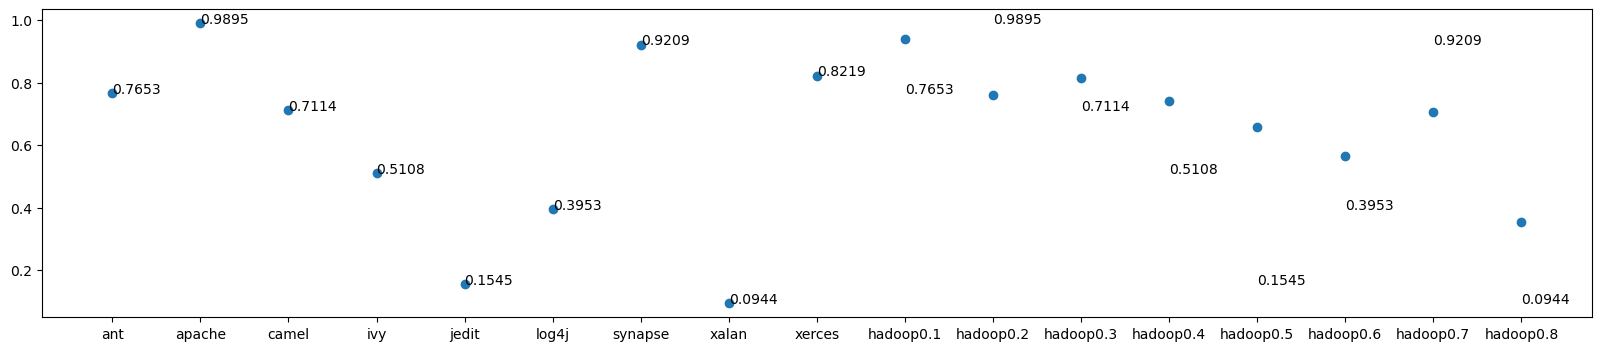
\includegraphics[width=0.99\linewidth]{figures/balance-C1.png}
        \caption{Balance C1}
        \label{fig:balance-c1}
    \end{subfigure}
    \begin{subfigure}{0.496\textwidth}
        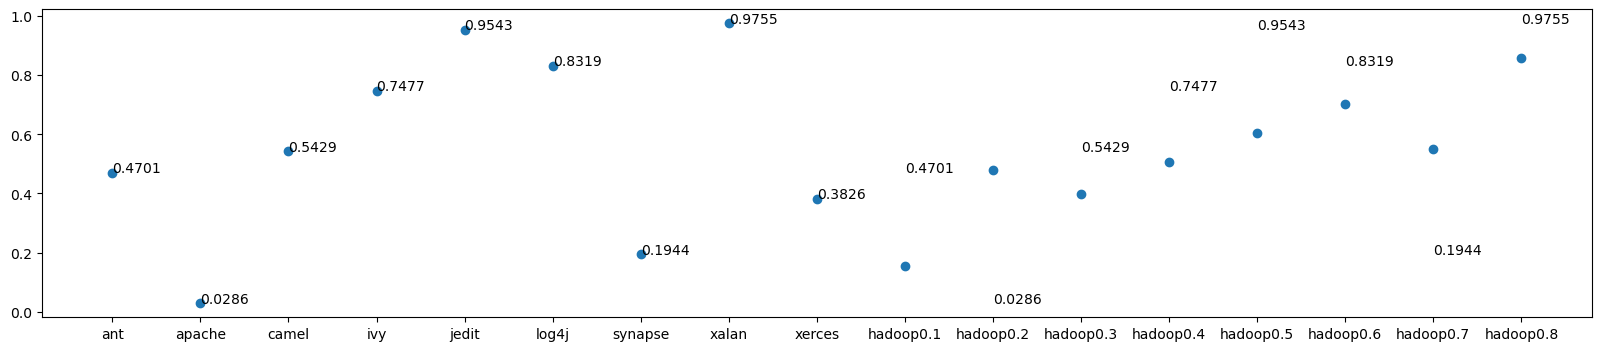
\includegraphics[width=0.99\linewidth]{figures/balance-C2.png}
        \caption{Balance C2}
        \label{fig:balance-c2}
    \end{subfigure}
    \caption{Balance Measures}
    \label{fig:balance}
\end{figure}

%%%%%%%%%%
\begin{figure}[h!]
    \centering
    \begin{subfigure}{0.496\textwidth}
        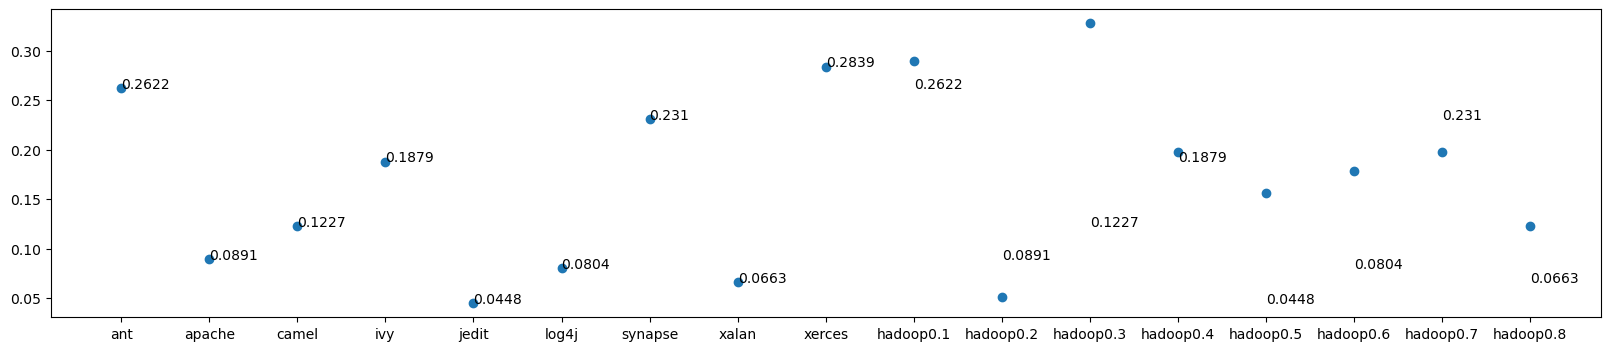
\includegraphics[width=0.99\textwidth]{figures/correlation-C2.png}
        \caption{Correlation C2}
        \label{fig:correlation-c2}
    \end{subfigure}
    \begin{subfigure}{0.496\textwidth}
        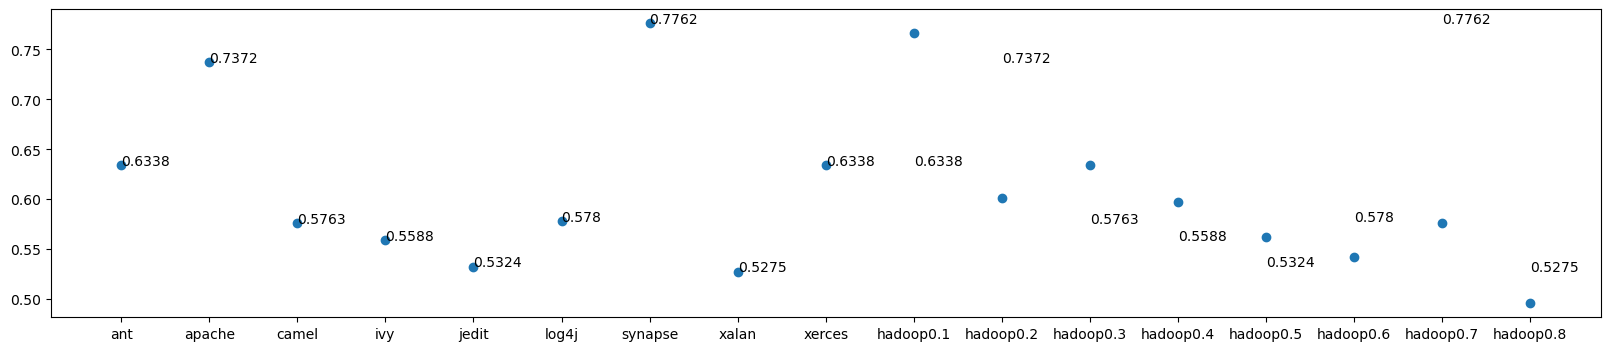
\includegraphics[width=0.99\textwidth]{figures/correlation-C3.png}
        \caption{Correlation C3}
        \label{fig:correlation-c3}
    \end{subfigure}
\end{figure}
\begin{figure}[h!]\ContinuedFloat
    \centering
    \begin{subfigure}{0.496\textwidth}
        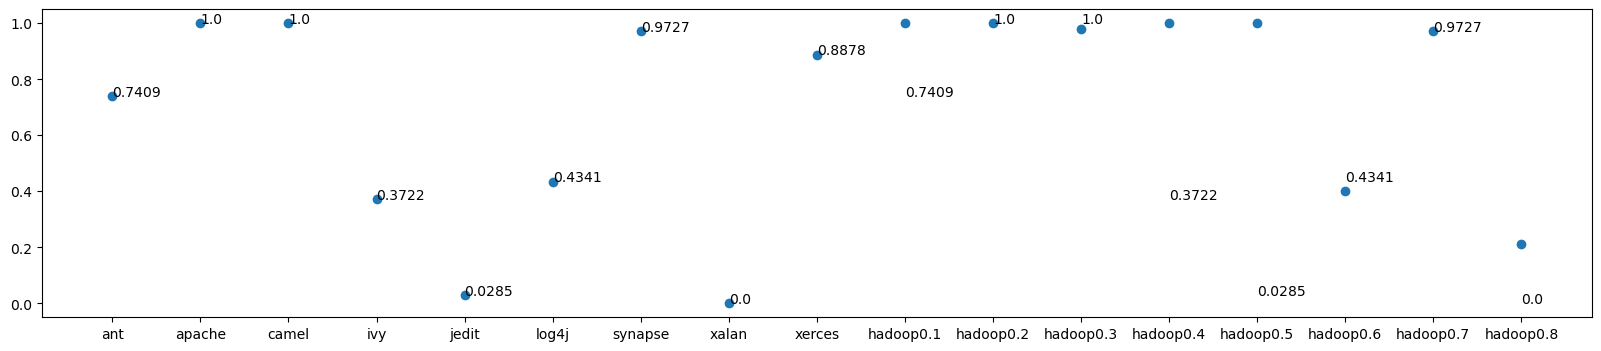
\includegraphics[width=0.99\textwidth]{figures/correlation-C4.png}
        \caption{Correlation C4}
        \label{fig:correlation-c4}
    \end{subfigure}
    \caption{Correlation Measures}
    \label{fig:correlation}
\end{figure}

%%%%%%%%%%
\begin{figure}[h!]
    \centering
    \begin{subfigure}{0.496\textwidth}
        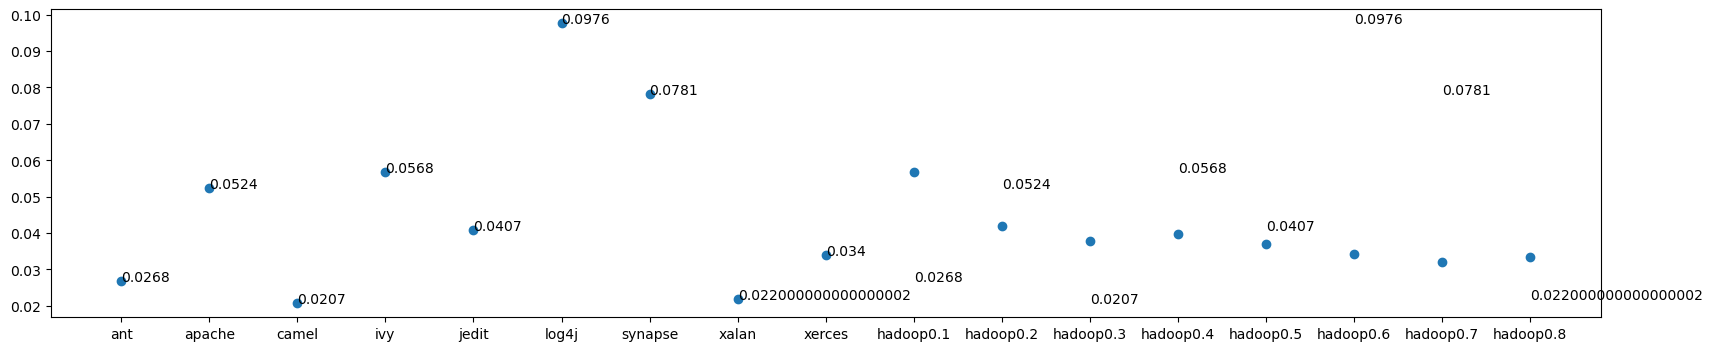
\includegraphics[width=0.99\textwidth]{figures/dimensionality-T2.png}
        \caption{Dimensionality T2}
        \label{fig:dimensionality-t2}
    \end{subfigure}
    \begin{subfigure}{0.496\textwidth}
        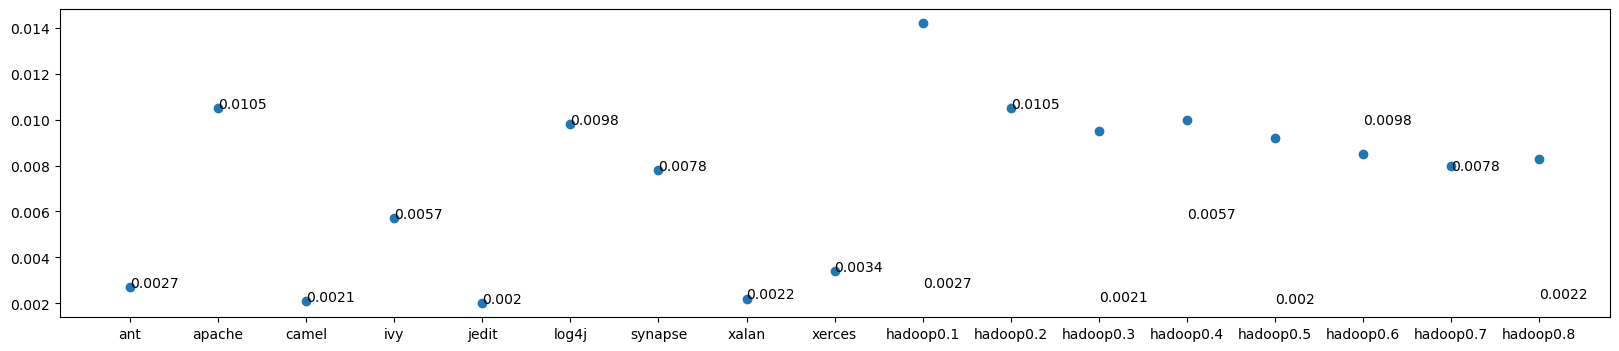
\includegraphics[width=0.99\textwidth]{figures/dimensionality-T3.png}
        \caption{Dimensionality T3}
        \label{fig:dimensionality-t3}
    \end{subfigure}
    \caption{Dimensionality Measures}
    \label{fig:dimensionality}
\end{figure}

%%%%%%%%%%
\begin{figure}[h!]
    \centering
    \begin{subfigure}{0.496\textwidth}
        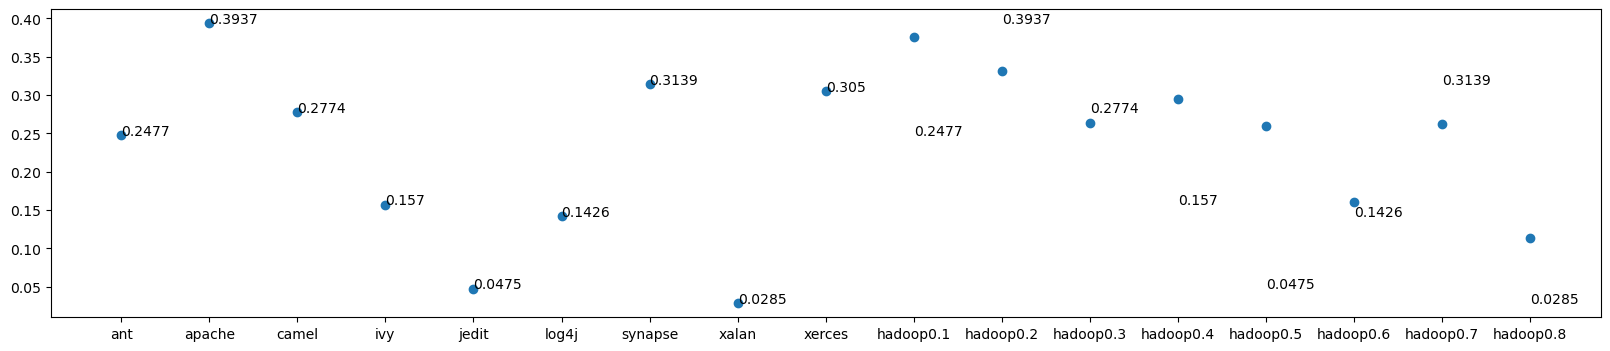
\includegraphics[width=0.99\textwidth]{figures/linearity-L1.png}
        \caption{Linearity L1}
        \label{fig:linearity-l1}
    \end{subfigure}
    \begin{subfigure}{0.496\textwidth}
        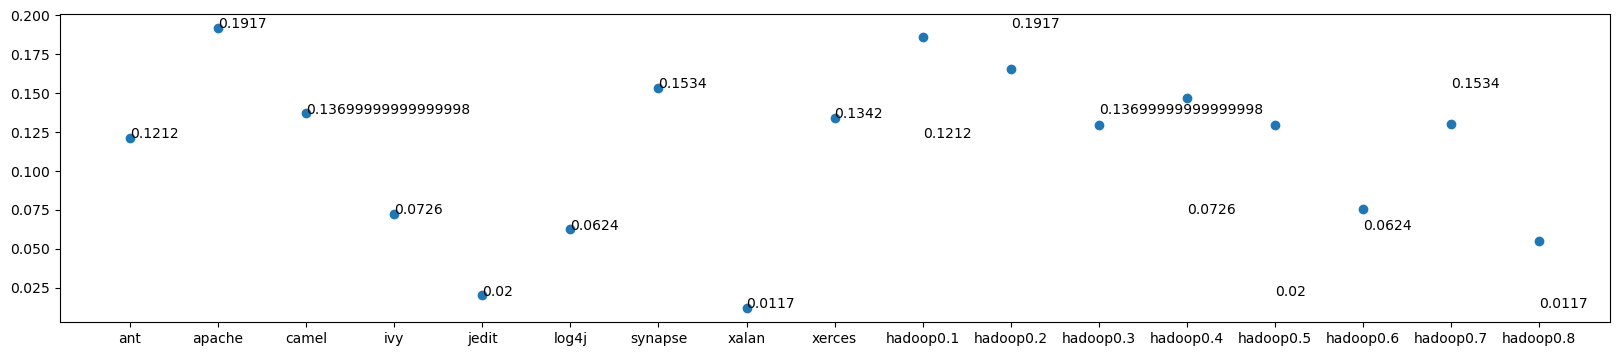
\includegraphics[width=0.99\textwidth]{figures/linearity-L2.png}
        \caption{Linearity L2}
        \label{fig:linearity-l2}
    \end{subfigure}
\end{figure}
\begin{figure}[h!]\ContinuedFloat
    \centering
    \begin{subfigure}{0.496\textwidth}
        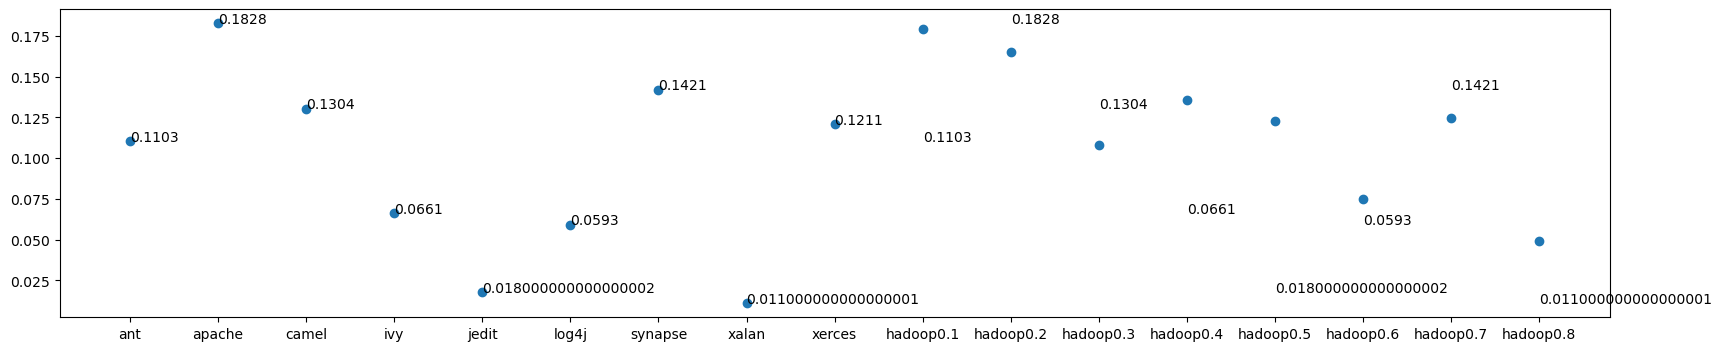
\includegraphics[width=0.99\textwidth]{figures/linearity-L3.png}
        \caption{Linearity L3}
        \label{fig:linearity-l3}
    \end{subfigure}
    \caption{Linearity Measures}
    \label{fig:linearity}
\end{figure}

%%%%%%%%%%
\begin{figure}[h!]
    \centering
    \begin{subfigure}{0.496\textwidth}
        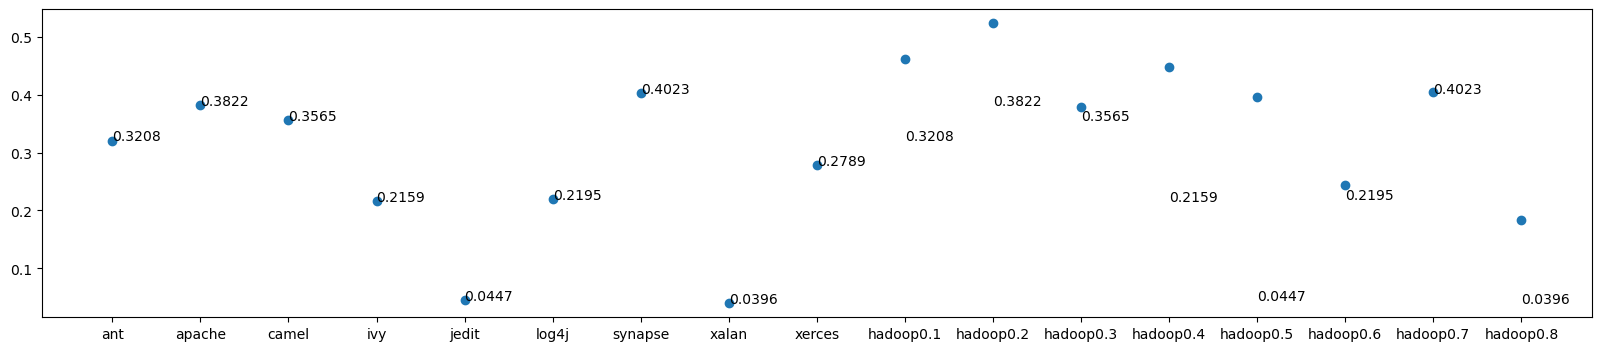
\includegraphics[width=0.99\textwidth]{figures/neighborhood-N1.png}
        \caption{Neighborhood N1}
        \label{fig:neighborhood-n1}
    \end{subfigure}
    \begin{subfigure}{0.496\textwidth}
        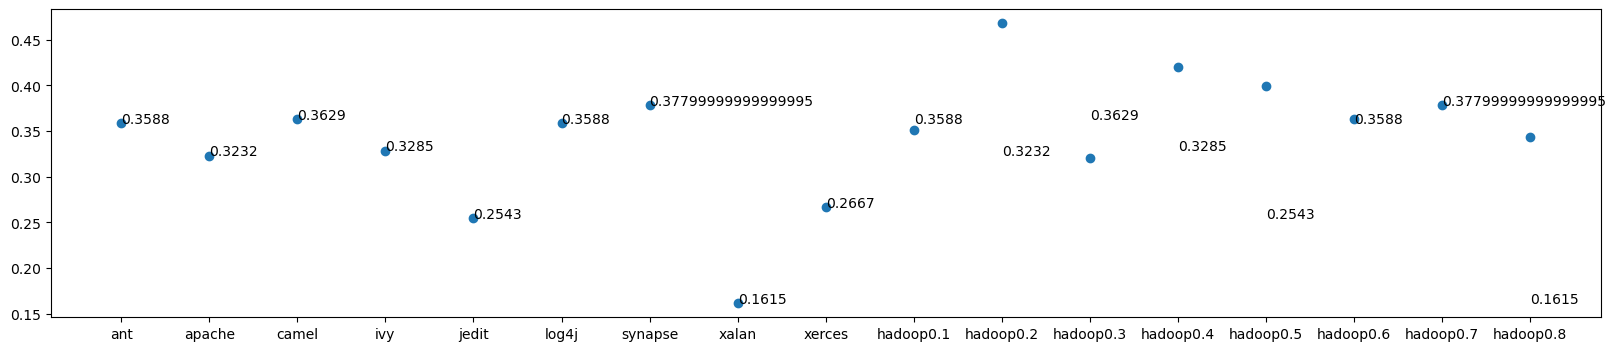
\includegraphics[width=0.99\textwidth]{figures/neighborhood-N2.png}
        \caption{Neighborhood N2}
        \label{fig:neighborhood-n2}
    \end{subfigure}
\end{figure}
\begin{figure}[h!]\ContinuedFloat
    \centering
    \begin{subfigure}{0.496\textwidth}
        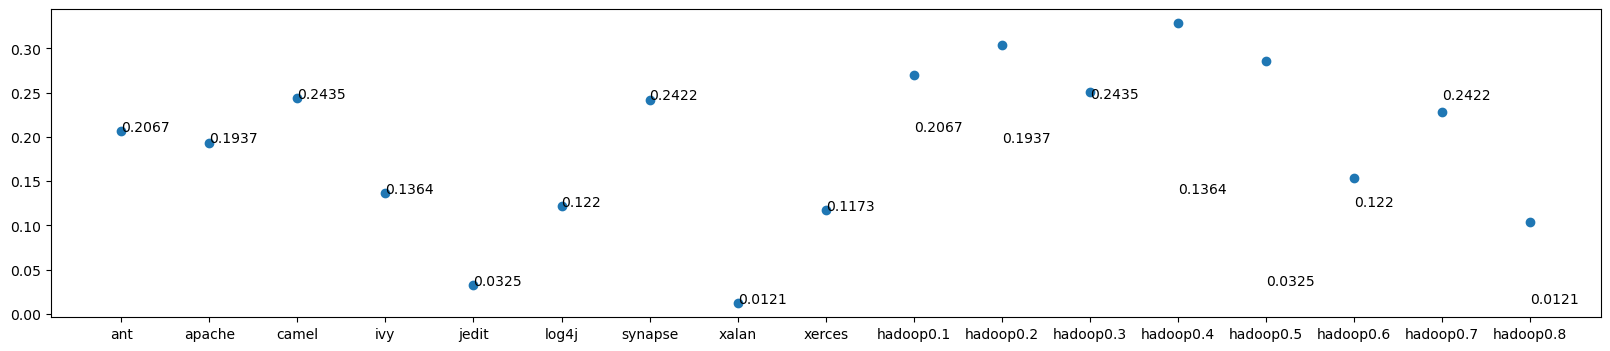
\includegraphics[width=0.99\textwidth]{figures/neighborhood-N3.png}
        \caption{Neighborhood N3}
        \label{fig:neighborhood-n3}
    \end{subfigure}
    \begin{subfigure}{0.496\textwidth}
        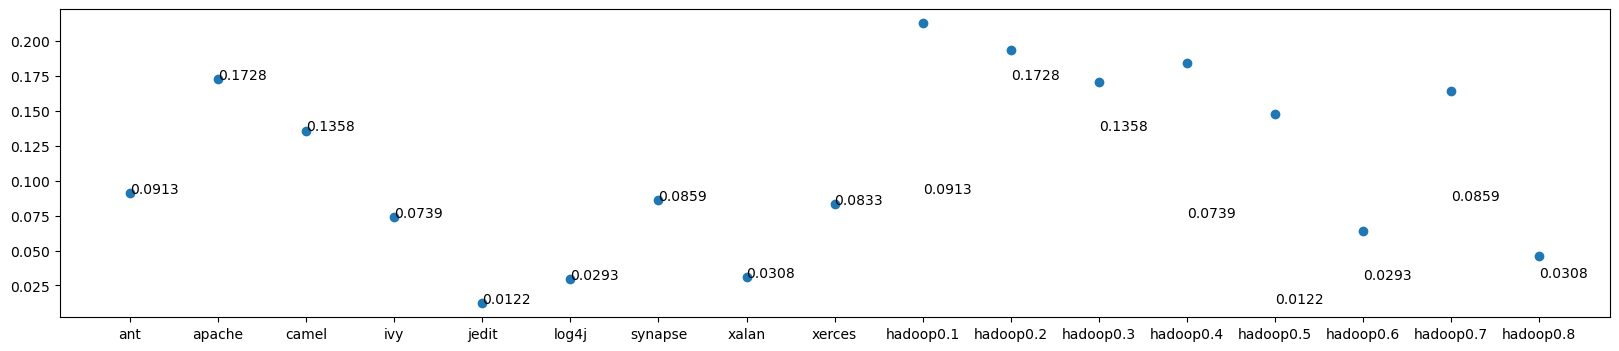
\includegraphics[width=0.99\textwidth]{figures/neighborhood-N4.png}
        \caption{Neighborhood N4}
        \label{fig:neighborhood-n4}
    \end{subfigure}
\end{figure}
\begin{figure}[h!]\ContinuedFloat
    \centering
    \begin{subfigure}{0.496\textwidth}
        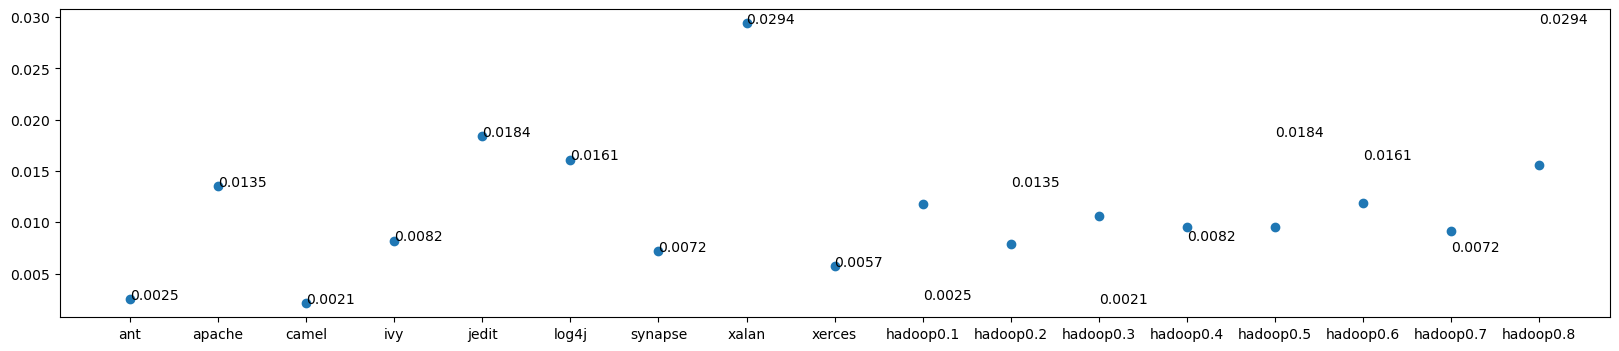
\includegraphics[width=0.99\textwidth]{figures/neighborhood-T1.png}
        \caption{Neighborhood T1}
        \label{fig:neighborhood-t1}
    \end{subfigure}
    \begin{subfigure}{0.496\textwidth}
        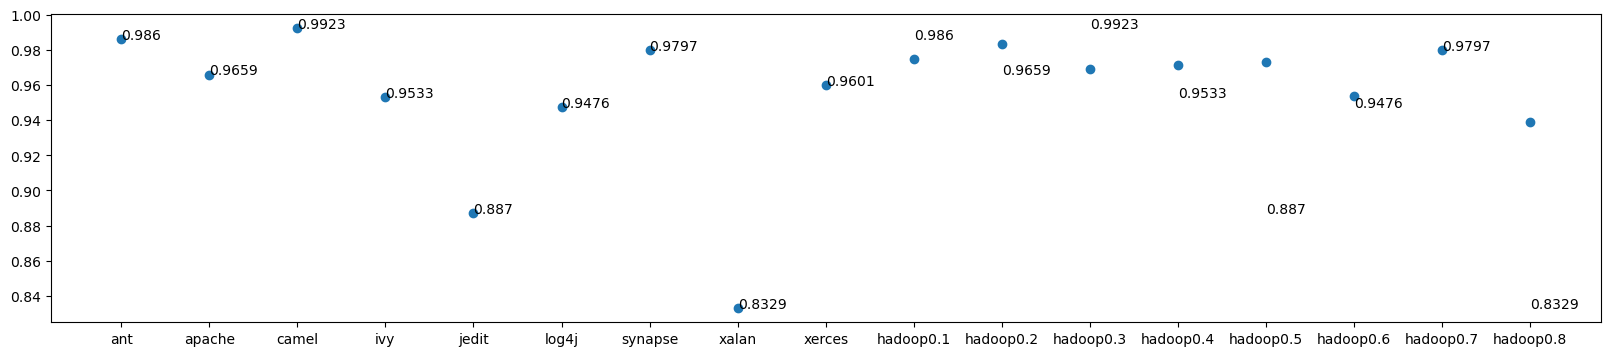
\includegraphics[width=0.99\textwidth]{figures/neighborhood-LSC.png}
        \caption{Neighborhood LSC}
        \label{fig:neighborhood-lsc}
    \end{subfigure}
    \caption{Neighborhood Measures}
    \label{fig:neighborhood}
\end{figure}

%%%%%%%%%%
\begin{figure}[h!]
    \centering
    \begin{subfigure}{0.496\textwidth}
        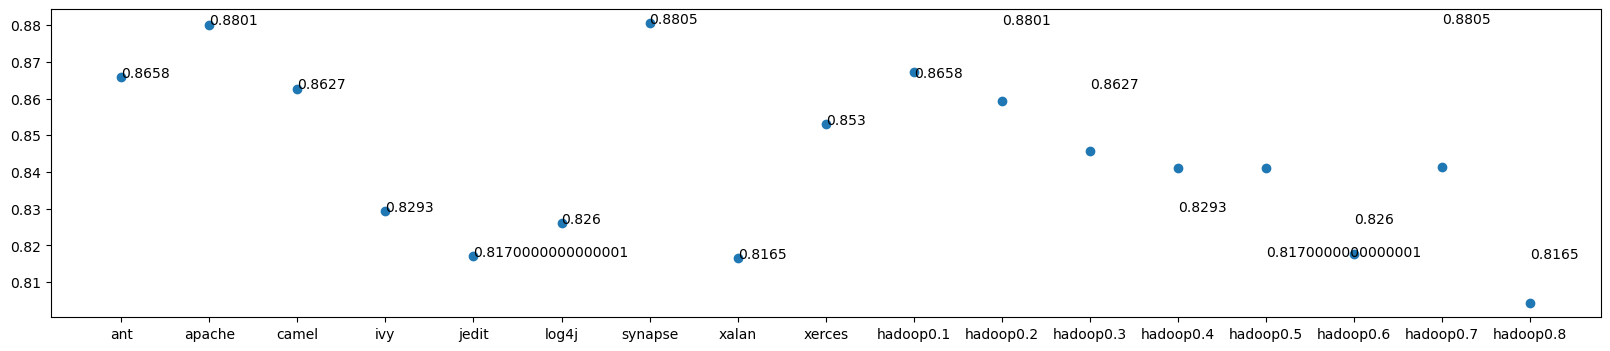
\includegraphics[width=0.99\textwidth]{figures/network-Density.png}
        \caption{Network Density}
        \label{fig:network-density}
    \end{subfigure}
    \begin{subfigure}{0.496\textwidth}
        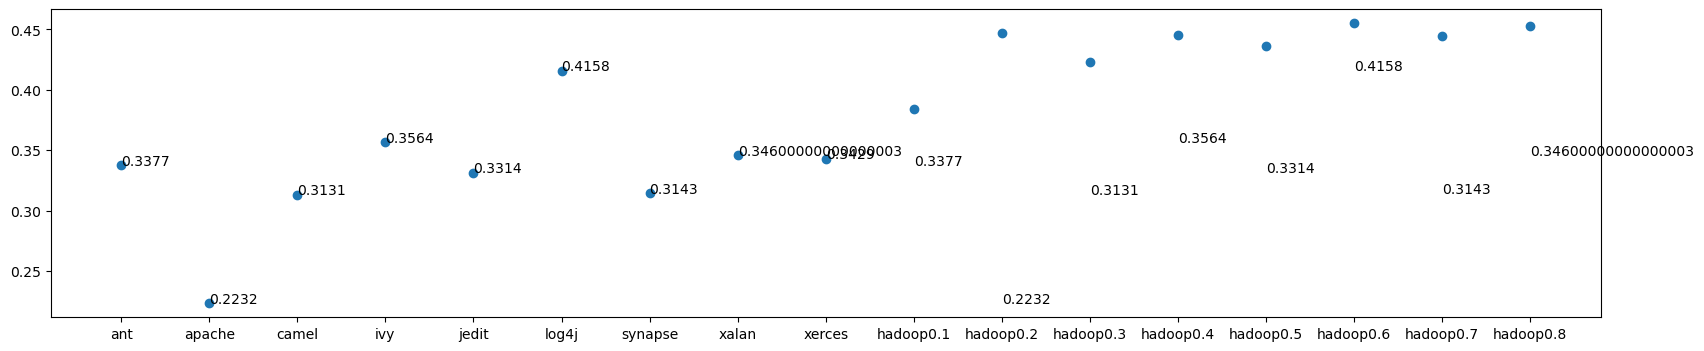
\includegraphics[width=0.99\textwidth]{figures/network-ClsCoef.png}
        \caption{Network ClsCoef}
        \label{fig:network-clscoef}
    \end{subfigure}
\end{figure}
\begin{figure}[h!]\ContinuedFloat
    \centering
    \begin{subfigure}{0.496\textwidth}
        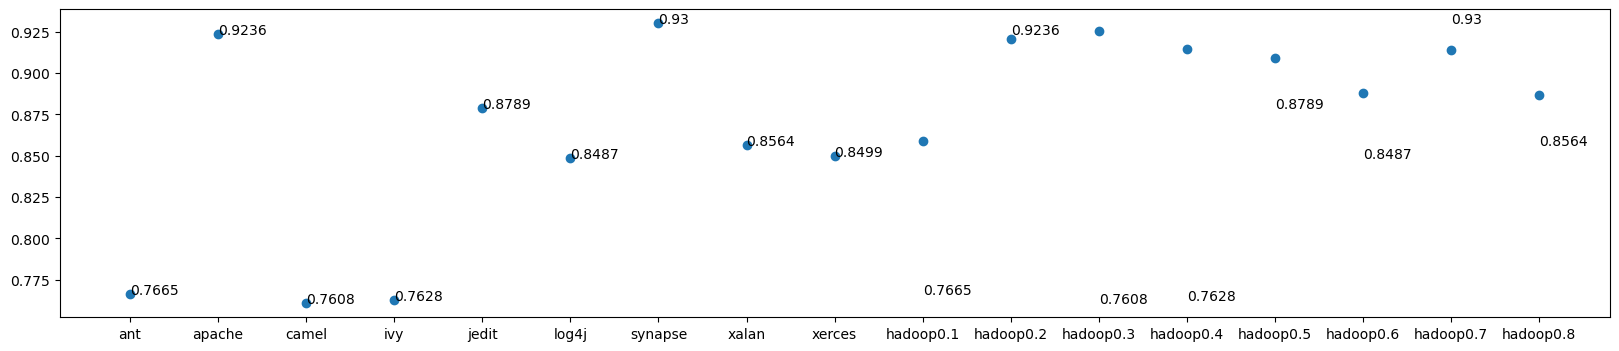
\includegraphics[width=0.99\textwidth]{figures/network-Hubs.png}
        \caption{Network Hubs}
        \label{fig:network-hubs}
    \end{subfigure}
    \caption{Network Measures}
    \label{fig:network}
\end{figure}

%%%%%%%%%%
\begin{figure}[h!]
    \centering
    \begin{subfigure}{0.496\textwidth}
        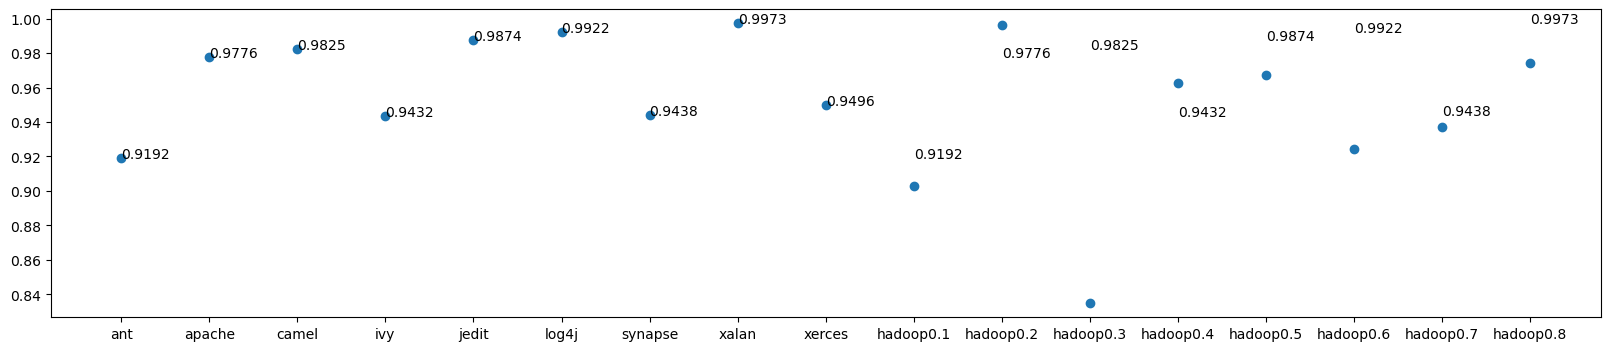
\includegraphics[width=0.99\textwidth]{figures/overlap-F1.png}
        \caption{Overlap F1}
        \label{fig:overlap-f1}
    \end{subfigure}
    \begin{subfigure}{0.496\textwidth}
        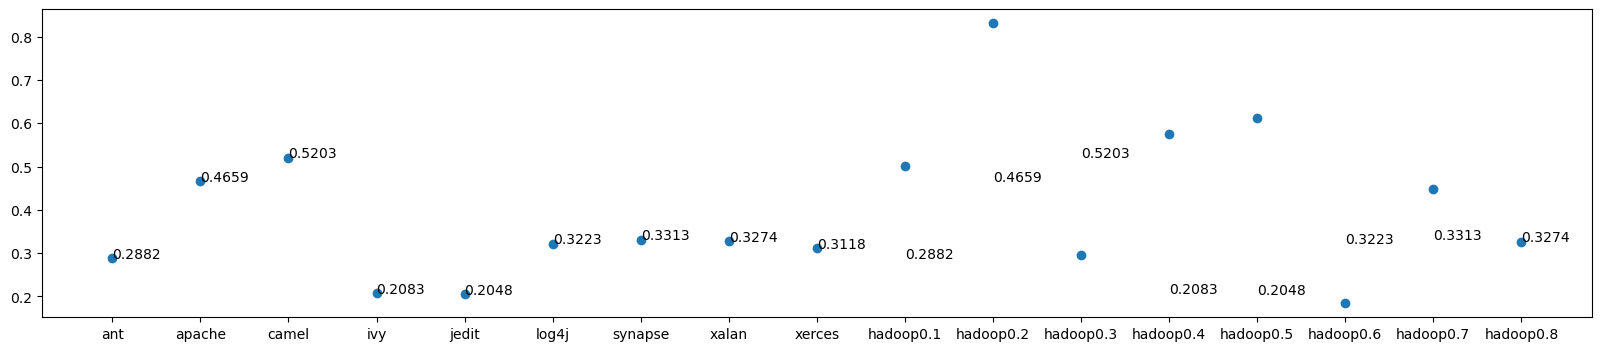
\includegraphics[width=0.99\textwidth]{figures/overlap-F1v.png}
        \caption{Overlap F1v}
        \label{fig:overlap-f1v}
    \end{subfigure}
\end{figure}
\begin{figure}[h!]\ContinuedFloat
    \centering
    \begin{subfigure}{0.496\textwidth}
        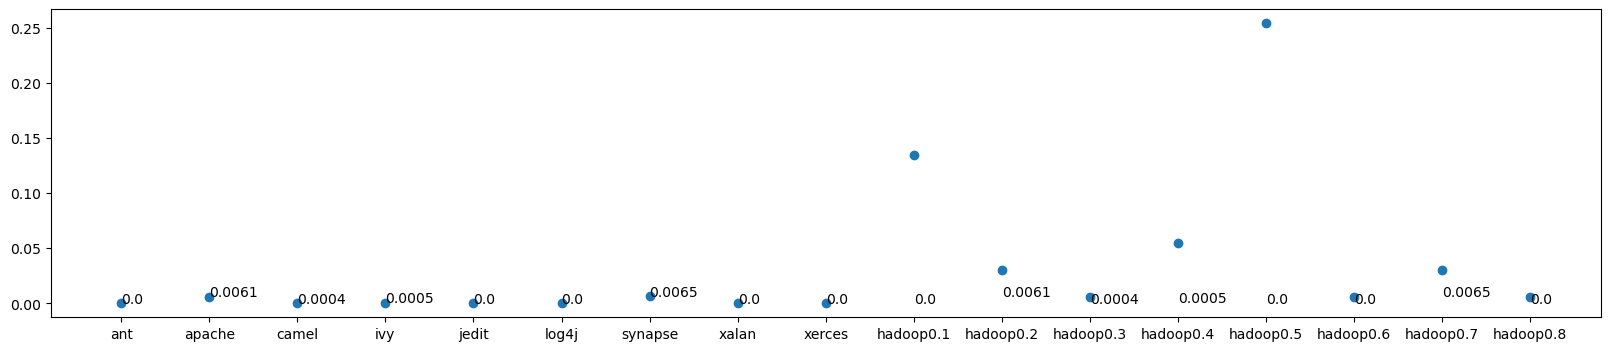
\includegraphics[width=0.99\textwidth]{figures/overlap-F2.png}
        \caption{Overlap F2}
        \label{fig:overlap-f2}
    \end{subfigure}
    \begin{subfigure}{0.496\textwidth}
        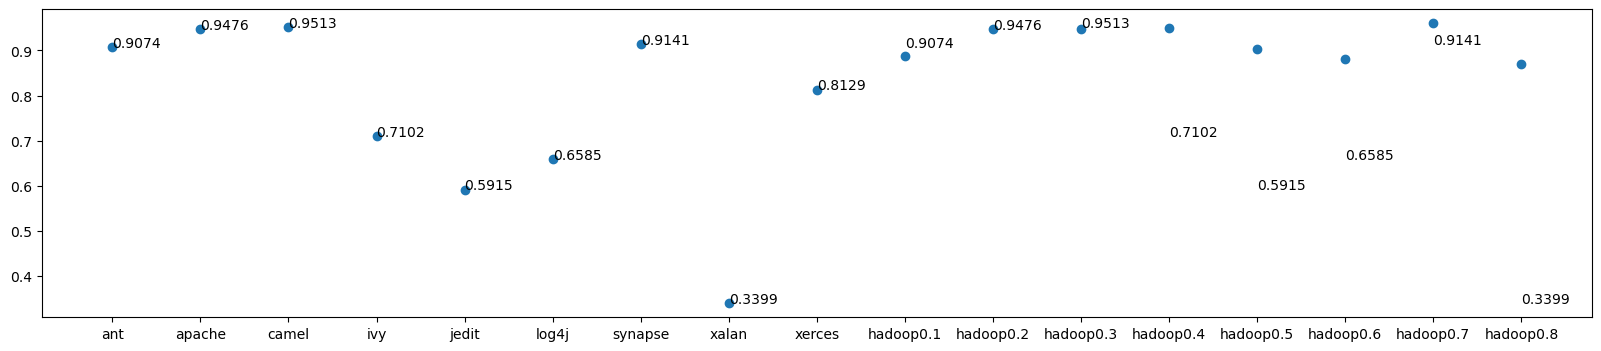
\includegraphics[width=0.99\textwidth]{figures/overlap-F3.png}
        \caption{Overlap F3}
        \label{fig:overlap-f3}
    \end{subfigure}
\end{figure}
\begin{figure}[h!]\ContinuedFloat
    \centering
    \begin{subfigure}{0.496\textwidth}
        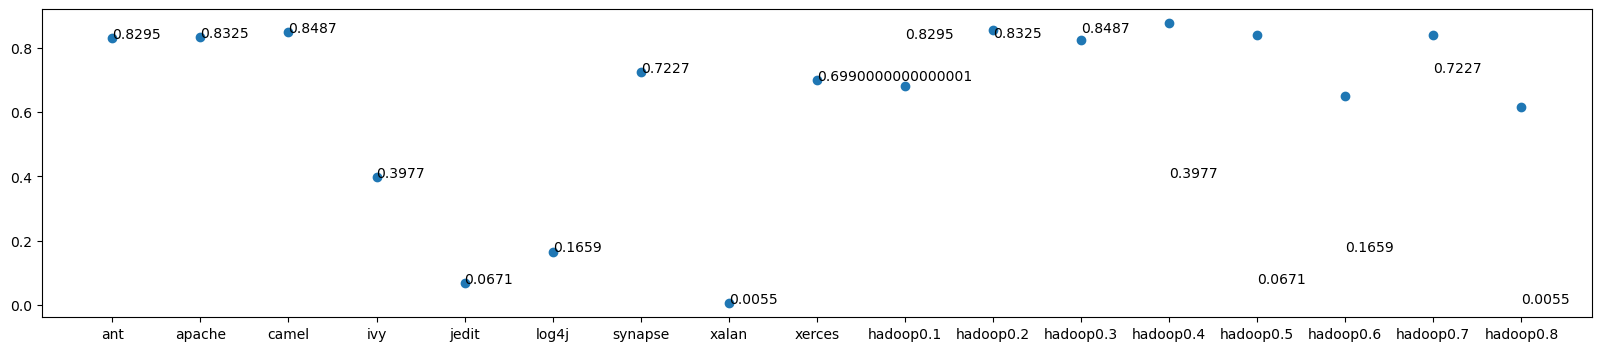
\includegraphics[width=0.99\textwidth]{figures/overlap-F4.png}
        \caption{Overlap F4}
        \label{fig:overlap-f4}
    \end{subfigure}
    \caption{Overlap Measures}
    \label{fig:overlap}
\end{figure}

%%%%%%%%%%
\begin{figure}[h!]
    \centering
    \begin{subfigure}{0.496\textwidth}
        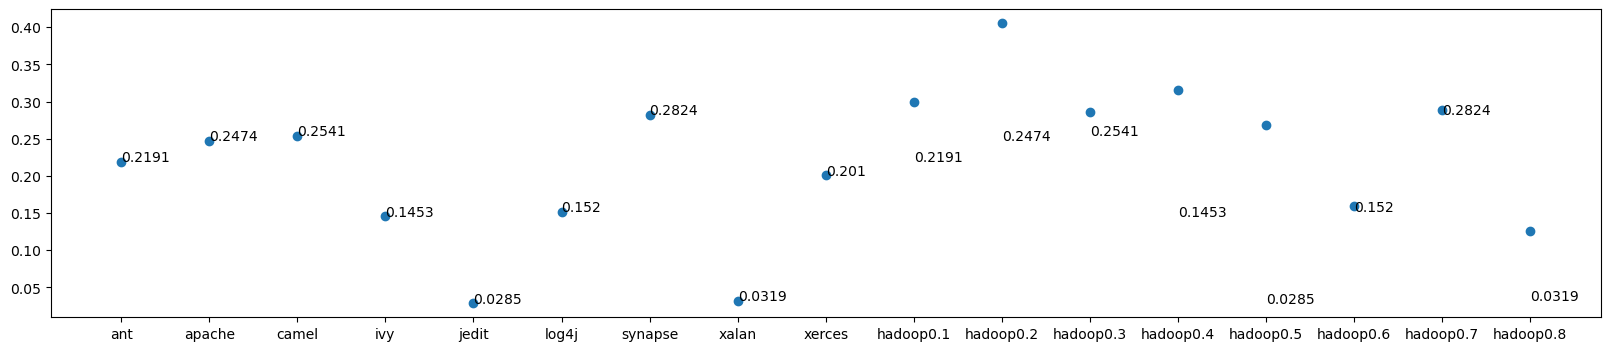
\includegraphics[width=0.99\textwidth]{figures/smoothness-S1.png}
        \caption{Smoothness S1}
        \label{fig:smoothness-s1}
    \end{subfigure}
    \begin{subfigure}{0.496\textwidth}
        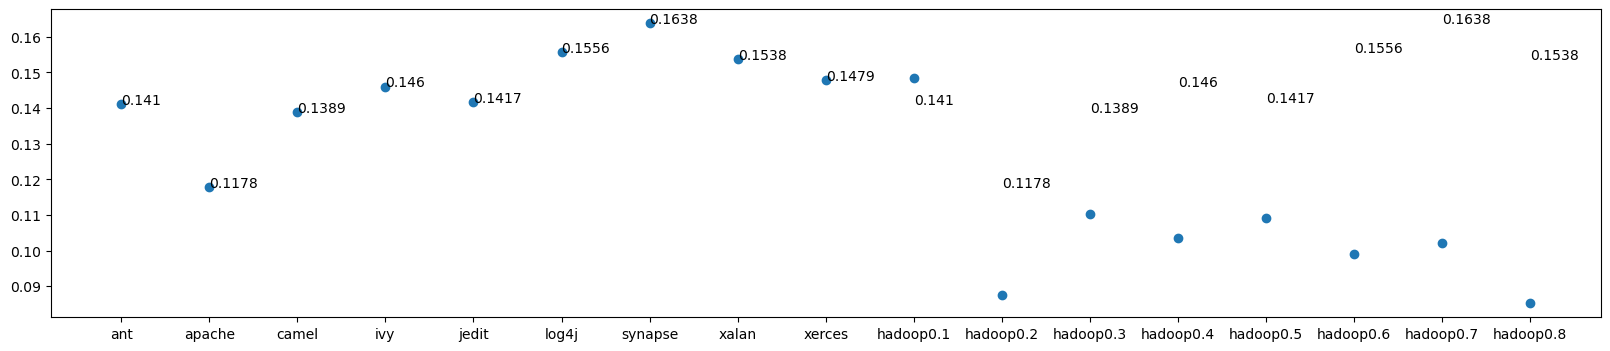
\includegraphics[width=0.99\textwidth]{figures/smoothness-S2.png}
        \caption{Smoothness S2}
        \label{fig:smoothness-s2}
    \end{subfigure}
\end{figure}
\begin{figure}[h!]\ContinuedFloat
    \centering
    \begin{subfigure}{0.496\textwidth}
        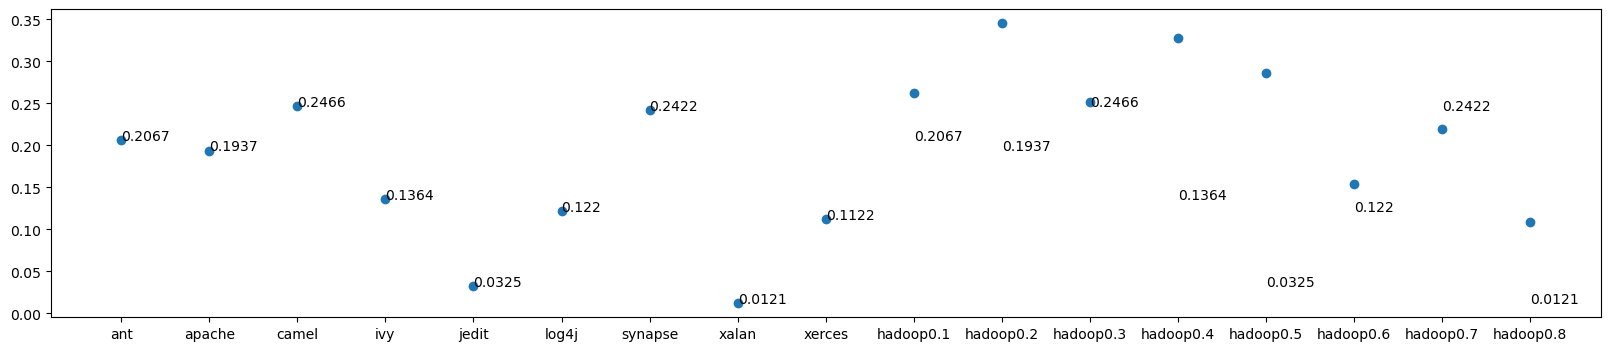
\includegraphics[width=0.99\textwidth]{figures/smoothness-S3.png}
        \caption{Smoothness S3}
        \label{fig:smoothness-s3}
    \end{subfigure}
    \begin{subfigure}{0.496\textwidth}
        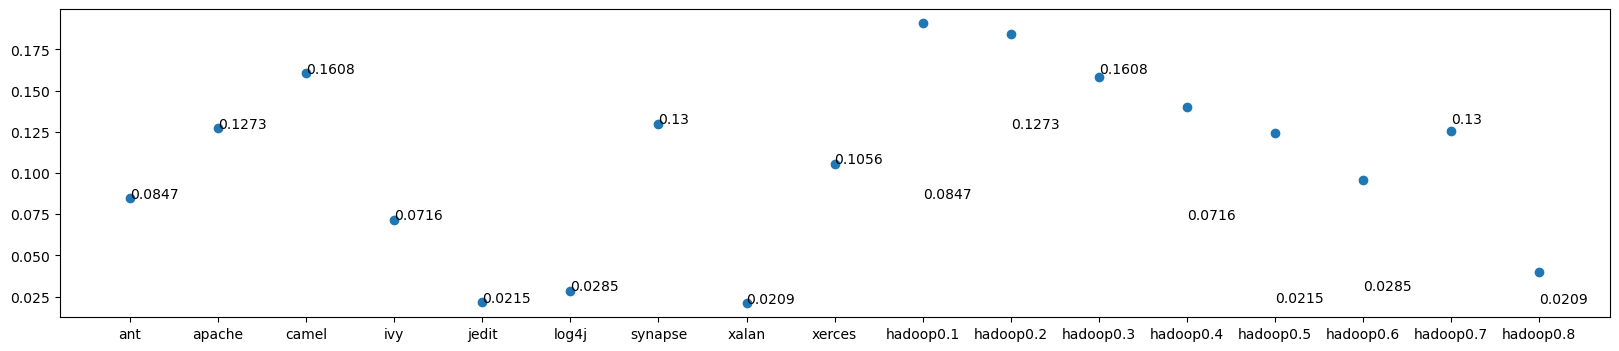
\includegraphics[width=0.99\textwidth]{figures/smoothness-S4.png}
        \caption{Smoothness S4}
        \label{fig:smoothness-s4}
    \end{subfigure}
    \caption{Smoothness Measures}
    \label{fig:smoothness}
\end{figure}

This way it is easier to compare results through datasets and metrics. To see 
the whole extent of the numerical values, see the tables at 
Appendix~\ref{chp:tables}. The data is summarized in tables \ref{sec:compl-oo} 
and \ref{sec:compl-hadoop}. To see the images in more detail (bigger) go to 
Appendix~\ref{chp:figures}, Section~\ref{sec:fig-compl-metrics}.

Further results are compared and discussed in Section~\ref{sec:compresults}.

%%%%%%%%%%%%%%%%%%%%%%%%%%%%%%%%%%%%%%%%%%%%%%%%%%%%%%%%%%%%%%%%%%%%%%
\subsection{Cross Validation Analysis}\label{sec:exp-kfold}

This experiment tries to find the impact of applying the $K$-fold 
Cross-Validation. It is a widely extended technique in data science that brings 
a solution to the problem of performing testing to a data set with no separate 
training data - the same instances in a given dataset should not be used for 
both training and testing a classifier at the same time, instead data can be 
divided so a portion is used for training and another separate portion for 
testing/validation. Cross validation allows us to estimate the performance of 
the model trained by the whole dataset dividing it into $k$ folds as follows:

\begin{itemize}
    \item Training set which is known data by the classifier, and used to train 
	it. It represents $k-1/k$ parts of the original set.
    \item Testing set, also known as validation set which corresponds to unseen 
	data for trained classifier used to test its performance. It usually is 
	$1/k$ of the original dataset.
\end{itemize}

Then, the average of carrying out $k$ iterations, same as the number of folds 
(parts/divisions) of the dataset, is calculated. On each iteration, the 
\textit{testing set} is rotated to another unused fold\footnote{The data in the 
different folds does not change throughout the cross validation process.} of the 
data - no testing set is repeated, which means that each fold is used only once 
for\textit{testing} purposes. 

The most common values for $k$ (folds) used in data science are 5 and 10. For 
this experiment, $k$ has been selected as $k=5$, as a common value of $k$ was 
needed for all experiments and some of the datasets did not have enough samples 
for a larger value of $k$.

The algorithm that analyses the performance of each fold and the calculates the 
mean performance can be simplified as the one explained in the 
Algorithm~\ref{alg:kfold}.

\begin{breakablealgorithm}
    \caption{Metrics Analysis on K-fold}
    \footnotesize
    \label{alg:kfold}
    \begin{algorithmic}[1]
        \Require $\mathcal{D}$ dataset
        \State inputs, targets $\leftarrow$ $\mathcal{D}$
    
        \State k $\leftarrow$ 5
        \State kf $\leftarrow$ kfold(k)
        \State splits $\leftarrow$ kf.split(inputs)
        
        \ForAll {$train_{i}$, $test_{i}$ in splits}
        	\State $x_{train}$, $x_{test}$ $\leftarrow$ inputs.get($train_{i}$), inputs.get($test_{i}$)
        	\State $y_{train}$, $y_{test}$ $\leftarrow$ targets.get($train_{i}$), targets.get($test_{i}$)
        	
        	\State clf $\leftarrow$ trainNetwork($x_{train}$, $y_{train}$)
        	
        	\State confusionMatrix($x_{test}$, $y_{test}$, clf)
        \EndFor
        \State calculateMeanPerformance(clf)
    \end{algorithmic}
\end{breakablealgorithm}

The Python script used for this experiment can be found in 
Appendix~\ref{chp:pythoncode}, Section~\ref{sec:exp-kfold-code}. It basically
separates a dataset into folds and calculates the performance metrics for each 
fold, to later on compute the mean value of those metrics for the entire dataset.

With the \textit{confusion matrix} other metrics are calculated such as 
$recall$, $MCC$, etc. Those metrics are then compared in Tables~\ref{tab:kfold} 
and~\ref{tab:kfold2}, for each specific dataset (to see the full extent of the 
comparison we refer to Section~\ref{sec:compresults}. For the sake of 
simplicity, only two tables of the aforementioned resulting datasets. 
Table~\ref{tab:kfold} shows the results obtained from Apache dataset.

\begin{center}
\begin{longtable}{ | r  l | c | c | c | c | c | c | c | }
\caption{Cross-Validation Results --- Apache Dataset}\label{tab:kfold} \\

\hline
\textbf{\emph{Fold}} & \textbf{\emph{Function}} & \emph{Precision} & \emph{Recall}  & \emph{Fall Out} & \emph{Balanced} & \emph{F1} & \emph{MCC} & \emph{AUC} \\
\hline
\endfirsthead
\hline
\multicolumn{9}{c}{\tablename\ \thetable\ -- \textit{Continued from previous page}} \\
\hline
\textbf{\emph{Fold}} & \textbf{\emph{Function}} & \emph{Precision} & \emph{Recall}  & \emph{Fall Out} & \emph{Balanced} & \emph{F1} & \emph{MCC} & \emph{AUC} \\
\hline
\endhead
\hline
\multicolumn{9}{r}{\textit{Continued on next page}}
\endfoot
\hline
\endlastfoot

\multirow{3}{*}{\textbf{1}} & \textbf{Naive Bayes} & 
0.4286 & 0.1579 & 0.200  & 0.4789 & 0.2308 & -0.0548 & 0.4789 \\
& \textbf{Decision Tree} & 
0.8235 & 0.7368 & 0.1500 & 0.7934 & 0.7778 &  0.5915 & 0.7934 \\
& \textbf{Nearest Centroid} &
0.3333 & 0.3158 & 0.6000 & 0.3579 & 0.3243 & -0.2850 & 0.3579 \\
\hline
\multirow{3}{*}{\textbf{2}} & \textbf{Naive Bayes} & 
0.5000 & 0.0800 & 0.1538 & 0.4631 & 0.1379 & -0.1142 & 0.4631 \\
& \textbf{Decision Tree} & 
0.8095 & 0.6800 & 0.3077 & 0.6862 & 0.7391 &  0.3552 & 0.6862 \\
& \textbf{Nearest Centroid} &
0.5000 & 0.1600 & 0.3077 & 0.4262 & 0.2424 & -0.1719 & 0.4262 \\
\hline
\multirow{3}{*}{\textbf{3}} & \textbf{Naive Bayes} & 
0.5000 & 0.0909 & 0.1250 & 0.4830 & 0.1538 & -0.0548 & 0.4830 \\
& \textbf{Decision Tree} & 
0.8462 & 0.5000 & 0.1250 & 0.6875 & 0.6286 &  0.3903 & 0.6875  \\
& \textbf{Nearest Centroid} &
0.4000 & 0.1818 & 0.3750 & 0.4034 & 0.2500 & -0.2166 & 0.4034 \\
\hline
\multirow{3}{*}{\textbf{4}} & \textbf{Naive Bayes} & 
0.3333 & 0.8182 & 0.6667 & 0.5758 & 0.4737 & 0.1515 & 0.5758 \\
& \textbf{Decision Tree} & 
0.5833 & 0.6364 & 0.1852 & 0.7256 & 0.6087 & 0.4402 & 0.7256 \\
& \textbf{Nearest Centroid} &
0.8000 & 0.7273 & 0.0741 & 0.8266 & 0.7619 & 0.6727 & 0.8266 \\
\hline
\multirow{3}{*}{\textbf{5}} & \textbf{Naive Bayes} & 
0.3043 & 1.0000 & 0.5161 & 0.7419 & 0.4667 & 0.3838 & 0.7419 \\
& \textbf{Decision Tree} & 
0.5000 & 1.0000 & 0.2258 & 0.8871 & 0.6667 & 0.6222 & 0.8871 \\
& \textbf{Nearest Centroid} &
0.4545 & 0.7143 & 0.1935 & 0.7604 & 0.5556 & 0.4451 & 0.7604 \\
\hline
\hline
% Mean
\multirow{3}{*}{\textbf{Mean}} & \textbf{Naive Bayes} & 
0.4132 & 0.4294 & 0.3323 & 0.5485 & 0.2926 & 0.0623 & 0.5485 \\
& \textbf{Decision Tree} & 
0.7125 & 0.7106 & 0.1987 & 0.7560 & 0.6842 & 0.4799 & 0.7560 \\
& \textbf{Nearest Centroid} &
0.4976 & 0.4198 & 0.3101 & 0.5549 & 0.4268 & 0.0889 & 0.5549 \\
\hline
\end{longtable}
\end{center}

The second example shown in Table~\ref{tab:kfold2} was obtained on the 
experiment performed over the Hadoop (v0.8) dataset.

\begin{center}
\begin{longtable}{ | r  l | c | c | c | c | c | c | c | }
\caption{Cross-Validation Results ---  Hadoop 0.8 Dataset}\label{tab:kfold2} \\

\hline
\textbf{\emph{Fold}} & \textbf{\emph{Function}} & \emph{Precision} & \emph{Recall}  & \emph{Fall Out} & \emph{Balanced} & \emph{F1} & \emph{MCC} & \emph{AUC} \\
\hline
\endfirsthead
\hline
\multicolumn{9}{c}{\tablename\ \thetable\ -- \textit{Continued from previous page}} \\
\hline
\textbf{\emph{Fold}} & \textbf{\emph{Function}} & \emph{Precision} & \emph{Recall}  & \emph{Fall Out} & \emph{Balanced} & \emph{F1} & \emph{MCC} & \emph{AUC} \\
\hline
\endhead
\hline
\multicolumn{9}{r}{\textit{Continued on next page}}
\endfoot
\hline
\endlastfoot

\multirow{3}{*}{\textbf{1}} & \textbf{Naive Bayes} & 
1.0000 & 0.1250 & 0.0000 & 0.5625 & 0.2222 & 0.3262  & 0.5625 \\
& \textbf{Decision Tree} & 
0.0000 & 0.0000 & 0.0250 & 0.4875 & 0.0000 & -0.0652 & 0.4875 \\
& \textbf{Nearest Centroid} &
0.1667 & 1.0000 & 1.0000 & 0.5000 & 0.2857 & 0.0000  & 0.5000 \\
\hline
\multirow{3}{*}{\textbf{2}} & \textbf{Naive Bayes} & 
0.0000 & 0.0000 & 0.1064 & 0.4468 & 0.0000 & -0.0497 & 0.4468 \\
& \textbf{Decision Tree} & 
0.0000 & 0.0000 & 0.1064 & 0.4468 & 0.0000 & -0.0497 & 0.4468 \\
& \textbf{Nearest Centroid} &
0.0208 & 1.0000 & 1.0000 & 0.5000 & 0.0408 & 0.0000 & 0.5000 \\
\hline
\multirow{3}{*}{\textbf{3}} & \textbf{Naive Bayes} & 
0.0000 & 0.0000 & 0.0851 & 0.4574 & 0.0000 & -0.0440 & 0.4574 \\
& \textbf{Decision Tree} & 
0.0000 & 0.0000 & 0.0851 & 0.4574 & 0.0000 & -0.0440 & 0.4574 \\
& \textbf{Nearest Centroid} &
0.0208 & 1.0000 & 1.0000 & 0.5000 & 0.0408 &  0.0000 & 0.5000 \\
\hline
\multirow{3}{*}{\textbf{4}} & \textbf{Naive Bayes} & 
0.3333 & 0.2500 & 0.0455 & 0.6023 & 0.2857 &  0.2335 & 0.6023 \\
& \textbf{Decision Tree} & 
0.0000 & 0.0000 & 0.0426 & 0.4787 & 0.0000 & -0.0304 & 0.4787 \\
& \textbf{Nearest Centroid} &
0.0000 & 0.0000 & 0.0227 & 0.4886 & 0.0000 & -0.0440 & 0.4886 \\
\hline
\multirow{3}{*}{\textbf{5}} & \textbf{Naive Bayes} & 
0.0000 & 0.0000 & 0.0000 & 0.5000 & 0.0000 & 0.0000 & 0.5000 \\
& \textbf{Decision Tree} & 
0.0000 & 0.0000 & 0.0000 & 0.5000 & 0.0000 & 0.0000 & 0.5000 \\
& \textbf{Nearest Centroid} &
0.0000 & 0.0000 & 0.0000 & 0.5000 & 0.0000 & 0.0000 & 0.5000 \\
\hline
\hline
% Mean
\multirow{3}{*}{\textbf{Mean}} & \textbf{Naive Bayes} & 
0.26667 & 0.0750 & 0.0474 & 0.5138 & 0.1016 & 0.0932 & 0.5138 \\
& \textbf{Decision Tree} & 
0.0000 & 0.0000 & 0.0484 & 0.4758 & 0.0000 & -0.0446 & 0.4758 \\
& \textbf{Nearest Centroid} &
0.0417 & 0.6000 & 0.6045 & 0.4977 & 0.0735 & -0.0088 & 0.4977 \\
\hline
\end{longtable}
\end{center}

The inner results of each fold are not evaluated when analyzing the results of 
the experiments, but that data could be used to understand how data metrics 
(including imbalance) affect classification. The objective evaluated in this 
paper is to see if the metrics obtained for each dataset have any relation with 
the performance of the classifiers. 

%%%%%%%%%%%%%%%%%%%%%%%%%%%%%%%%%%%%%%%%%%%%%%%%%%%%%%%%%%%%%%%%%%%%%%
\subsection{Imbalance Experimental Work}

After experimenting with cross-validation, we now focus on if filters applied 
to the dataset have any effect on the quality of the trained classifier. In this
case, it is carried out by applying imbalance filters to the folds in the 
datasets (see Section~\ref{sec:imbtechniques} for more information on imbalance 
filters). Here, the following techniques were used in the experiments:

\begin{description}
    \item [Undersampling] Removing samples from majority class.
    \item [Oversampling] Creating new samples in the minority class.
\end{description}

%%%%%%%%%%%%%%%%%%%%%%%%%%%%%%%%%%%%%%%%%%%%%%%%%%%%%%%%%%%%
\subsubsection{Undersampling with Cross Validation}
\label{sec:kfoldunder}

For this experiment, one undersampling algorithm is applied 
(\ref{nearmiss}) to see how folds are affected by removing majority class 
samples, and therefore, looking at how it impacts the classification algorithm. 

The undersampling technique is not done on the whole dataset in advance, only 
the training folds are the ones that the undersampling algorithm is applied. 

The $k$ value chosen for cross validation is $k=5$. A simplification
of the procedure followed by this experiment can be found in the 
Algorithm~\ref{alg:kfoldunder}.

\begin{breakablealgorithm}
    \caption{Undersampling with Cross-Validation}
    \label{alg:kfoldunder}
    \begin{algorithmic}[1]
        \Require $\mathcal{D}$ dataset
        \State inputs, targets $\leftarrow$ $\mathcal{D}$
    
        \State k $\leftarrow$ 5
        \State kf $\leftarrow$ kfold(k)
        \State splits $\leftarrow$ kf.split(inputs)
        
        \State samplingStrategy $\leftarrow$ {0:50, 1:50} \Comment{Binary class with a post undersampling distribution of 50-50}
        \State randomState $\leftarrow$ 42
        
        \ForAll {$train_{i}$, $test_{i}$ in splits}
        	\State $x_{train}$, $x_{test}$ $\leftarrow$ inputs.get($train_{i}$), inputs.get($test_{i}$)
        	\State $y_{train}$, $y_{test}$ $\leftarrow$ targets.get($train_{i}$), targets.get($test_{i}$)
        	
        	\State X, Y = makeImbalance(
        	\State \quad $x_{train}$, $y_{train}$,
        	\State \quad samplingStrategy,
        	\State \quad randomState
        	\State )
        	
        	\State clf $\leftarrow$ classifier(NearMiss(2), GaussianNB())
        	\State clf $\leftarrow$ trainNetwork(X, Y)
        	
        	\State confusionMatrix($x_{test}$, $y_{test}$, clf)
        \EndFor
        \State calculateMeanPerformance(clf)
    \end{algorithmic}
\end{breakablealgorithm}

Similarly to the previous experiment, the following classification algorithms 
were used to measure performance of the alterations done on the dataset, i.e., 
(1) Naive Bayes (Gaussian), (2) Decision Tree and (3) kNN Nearest Centroid.

The experiment creates the same tables obtained in 
experiment~\ref{sec:exp-kfold}, that is why sharing all the resulting tables of 
this experiment would be unnecessary - the results evaluated here can be found 
in Section~\ref{sec:compresults}. That is why only two of them have been 
included into this dissertation. The Apache dataset experiment (see 
Table~\ref{tab:kfoldunder}).

\begin{center}
\begin{longtable}{ | r  l | c | c | c | c | c | c | c | }
\caption{Cross-validation with Undersampling Results --- Apache dataset}
\label{tab:kfoldunder} 
\\
\hline
\textbf{\emph{Fold}} & \textbf{\emph{Function}} & 
\emph{Precision} & \emph{Recall}  & \emph{Fall Out} & 
\emph{Balanced} & \emph{F1} & \emph{MCC} & \emph{AUC} \\
\hline
\endfirsthead
\hline
\multicolumn{9}{c}{\tablename\ \thetable\ -- \textit{Continued from previous page}} \\
\hline
\textbf{\emph{Fold}} & \textbf{\emph{Function}} & 
\emph{Precision} & \emph{Recall}  & \emph{Fall Out} & 
\emph{Balanced} & \emph{F1} & \emph{MCC} & \emph{AUC} \\
\hline
\endhead
\hline
\multicolumn{9}{r}{\textit{Continued on next page}}
\endfoot
\hline
\endlastfoot
\hline

\multirow{3}{*}{\textbf{1}} & \textbf{Naive Bayes} & 
0.5556 & 0.8824 & 0.5455 & 0.6684 & 0.6818 &  0.3620 & 0.6684 \\
& \textbf{Decision Tree} & 
0.7000 & 0.8235 & 0.2727 & 0.7754 & 0.7568 &  0.5464 & 0.7754 \\
& \textbf{Nearest Centroid} &
0.4167 & 0.2941 & 0.3182 & 0.4880 & 0.3448 & -0.0259 & 0.4880 \\
\hline
\multirow{3}{*}{\textbf{2}} & \textbf{Naive Bayes} & 
0.5500 & 0.7333 & 0.3913 & 0.6710 & 0.6286 &  0.3348 & 0.6710 \\
& \textbf{Decision Tree} & 
0.5500 & 0.7333 & 0.3913 & 0.6710 & 0.6286 &  0.3348 & 0.6710 \\
& \textbf{Nearest Centroid} &
0.3571 & 0.3333 & 0.3913 & 0.4710 & 0.3448 & -0.0587 & 0.4710  \\
\hline
\multirow{3}{*}{\textbf{3}} & \textbf{Naive Bayes} & 
0.7586 & 0.8800 & 0.5385 & 0.6708 & 0.8148 & 0.3811 & 0.6708 \\
& \textbf{Decision Tree} & 
0.8421 & 0.6400 & 0.2308 & 0.7046 & 0.7273 & 0.3883 & 0.7046 \\
& \textbf{Nearest Centroid} &
0.7000 & 0.2800 & 0.2308 & 0.5246 & 0.4000 & 0.0530 & 0.5246 \\
\hline
\multirow{3}{*}{\textbf{4}} & \textbf{Naive Bayes} & 
0.6667 & 0.7273 & 0.1481 & 0.7896 & 0.6957 & 0.5650 & 0.7896 \\
& \textbf{Decision Tree} & 
0.6667 & 0.7273 & 0.1481 & 0.7896 & 0.6957 & 0.5650 & 0.7896 \\
& \textbf{Nearest Centroid} &
0.3077 & 0.3636 & 0.3333 & 0.5152 & 0.3333 & 0.0290 & 0.5152 \\
\hline
\multirow{3}{*}{\textbf{5}} & \textbf{Naive Bayes} & 
0.5000 & 0.5625 & 0.4091 & 0.5767 & 0.5294 & 0.1517 & 0.5767 \\
& \textbf{Decision Tree} & 
0.6316 & 0.7500 & 0.3182 & 0.7159 & 0.6857 & 0.4264 & 0.7159 \\
& \textbf{Nearest Centroid} &
0.5556 & 0.3125 & 0.1818 & 0.5653 & 0.4000 & 0.1518 & 0.5653 \\
\hline
\multirow{3}{*}{\textbf{Mean}} & \textbf{Naive Bayes} & 
0.5928 & 0.6662 & 0.3917 & 0.6372 & 0.6059 & 0.2992 & 0.6372 \\
& \textbf{Decision Tree} & 
0.6781 & 0.7348 & 0.2722 & 0.7313 & 0.6988 & 0.4522 & 0.7313 \\
& \textbf{Nearest Centroid} &
0.4674 & 0.3167 & 0.2911 & 0.5128 & 0.3646 & 0.0298 & 0.5128 \\
\hline
\end{longtable}
\end{center}

And the result obtained on the same experiment for the Hadoop (v0.8)
experiment (see Table~\ref{tab:kfoldunder2}).

\begin{center}
\begin{longtable}{ | r  l | c | c | c | c | c | c | c | }
\caption{Cross-validation with Undersampling Results --- Hadoop 0.8}\label{tab:kfoldunder2} \\
\hline
\textbf{\emph{Fold}} & \textbf{\emph{Function}} & 
\emph{Precision} & \emph{Recall}  & \emph{Fall Out} & 
\emph{Balanced} & \emph{F1} & \emph{MCC} & \emph{AUC} \\
\hline
\endfirsthead
\hline
\multicolumn{9}{c}{\tablename\ \thetable\ -- \textit{Continued from previous page}} \\
\hline
\textbf{\emph{Fold}} & \textbf{\emph{Function}} & 
\emph{Precision} & \emph{Recall}  & \emph{Fall Out} & 
\emph{Balanced} & \emph{F1} & \emph{MCC} & \emph{AUC} \\
\hline
\endhead
\hline
\multicolumn{9}{r}{\textit{Continued on next page}}
\endfoot
\hline
\endlastfoot
\hline

\multirow{3}{*}{\textbf{1}} & \textbf{Naive Bayes} & 
0.1429 & 0.5000 & 0.1304 & 0.6848 & 0.2222 &  0.2092 & 0.6848 \\
& \textbf{Decision Tree} & 
0.1053 & 1.0000 & 0.3696 & 0.8152 & 0.1905 &  0.2576 & 0.8152 \\
& \textbf{Nearest Centroid} &
0.0345 & 0.5000 & 0.6087 & 0.4457 & 0.0645 & -0.0444 & 0.4457 \\
\hline
\multirow{3}{*}{\textbf{2}} & \textbf{Naive Bayes} & 
0.0000 & 0.0000 & 0.2667 & 0.3667 & 0.0000 & -0.1491 & 0.3667 \\
& \textbf{Decision Tree} & 
0.0833 & 0.3333 & 0.2444 & 0.5444 & 0.1333 &  0.0497 & 0.5444 \\
& \textbf{Nearest Centroid} &
0.0952 & 0.6667 & 0.4222 & 0.6222 & 0.1667 &  0.1193 & 0.6222 \\
\hline
\multirow{3}{*}{\textbf{3}} & \textbf{Naive Bayes} & 
0.0833 & 0.5000 & 0.2391 & 0.6304 & 0.1429 &  0.1204 & 0.6304\\
& \textbf{Decision Tree} & 
0.0000 & 0.0000 & 0.3261 & 0.3370 & 0.0000 & -0.1406 & 0.3370 \\
& \textbf{Nearest Centroid} &
0.0000 & 0.0000 & 0.4348 & 0.2826 & 0.0000 & -0.1762 & 0.2826 \\
\hline
\multirow{3}{*}{\textbf{4}} & \textbf{Naive Bayes} & 
0.1333 & 0.3333 & 0.3095 & 0.5119 & 0.1905 &  0.0170 & 0.5119 \\
& \textbf{Decision Tree} & 
0.1765 & 0.5000 & 0.3333 & 0.5833 & 0.2609 &  0.1153 & 0.5833 \\
& \textbf{Nearest Centroid} &
0.0625 & 0.1667 & 0.3571 & 0.4048 & 0.0909 & -0.1336 & 0.4048 \\
\hline
\multirow{3}{*}{\textbf{5}} & \textbf{Naive Bayes} & 
0.0000 & 0.0000 & 0.1556 & 0.4222 & 0.0000 & -0.1067 & 0.4222 \\
& \textbf{Decision Tree} & 
0.2000 & 0.6667 & 0.1778 & 0.7444 & 0.3077 &  0.2914 & 0.7444 \\
& \textbf{Nearest Centroid} &
0.0000 & 0.0000 & 0.2444 & 0.3778 & 0.0000 & -0.1408 & 0.3778 \\
\hline
\multirow{3}{*}{\textbf{Mean}} & \textbf{Naive Bayes} & 
0.0719 & 0.2667 & 0.2203 & 0.5232 & 0.1111 &  0.0182 & 0.5232 \\
& \textbf{Decision Tree} & 
0.1130 & 0.5000 & 0.2902 & 0.6049 & 0.1785 &  0.1147 & 0.6049 \\
& \textbf{Nearest Centroid} &
0.0384 & 0.2667 & 0.4134 & 0.4266 & 0.0644 & -0.0751 & 0.4266 \\
\hline
\end{longtable}
\end{center}

As it has been mentioned in Section~\ref{nearmiss}, there are several versions 
of \textit{Near Miss} algorithm. For this experiment it was used \textit{version 
2}. This undersampling algorithm selects the majority class samples with the 
least average distance to the 3 farthest minority class samples.

The analysis of the metrics obtained are discussed in 
Section~\ref{sec:compresults}.

%%%%%%%%%%%%%%%%%%%%%%%%%%%%%%%%%%%%%%%%%%%%%%%%%%%%%%%%%%%%
\subsubsection{Oversampling with Cross Validation}

In this experiment, similarly to Section~\ref{sec:kfoldunder}, an imbalance 
filter is used. In this case, the oversampling technique is implemented and is 
later on compared to other experiment results (see 
Section~\ref{sec:compresults}).

The technique has been applied to the different folds of the dataset, not to the
entire data. Once again, the dataset is divided into $k=5$ folds. 

The logic of the Python code experiment is summarized in 
Algorithm~\ref{alg:kfoldover}. The difference with the undersampling 
Algorithm~\ref{alg:kfoldunder} is that uses the SMOTE technique (see 
Section~\ref{smote}) instead of \textit{Near Miss} undersampling technique.

\begin{breakablealgorithm}
    \caption{Oversampling and K-fold on classification performance}
    \footnotesize
    \label{alg:kfoldover}
    \begin{algorithmic}[1]
        \Require $\mathcal{D}$ dataset
        \State inputs, targets $\leftarrow$ $\mathcal{D}$
    
        \State k $\leftarrow$ 5
        \State kf $\leftarrow$ kfold(k)
        \State splits $\leftarrow$ kf.split(inputs)
        
        \ForAll {$train_{i}$, $test_{i}$ in splits}
        	\State $x_{train}$, $x_{test}$ $\leftarrow$ inputs.get($train_{i}$), inputs.get($test_{i}$)
        	\State $y_{train}$, $y_{test}$ $\leftarrow$ targets.get($train_{i}$), targets.get($test_{i}$)
        	
        	\State clf $\leftarrow$ classifier(SMOTE(), GaussianNB())
        	\State clf $\leftarrow$ trainNetwork($x_{train}$, $y_{train}$)
        	
        	\State confusionMatrix($x_{test}$, $y_{test}$, clf)
        \EndFor
        \State calculateMeanPerformance(clf)
    \end{algorithmic}
\end{breakablealgorithm}

The classifiers used for this experiment are - (1) Naive Bayes (Gaussian); 
(2) Decision Tree; and (3) kNN Nearest Centroid.

Next we show two of the results obtained, fhe first one is the result on the 
Apache dataset (see Table~\ref{tab:kfoldover-apache}).

\begin{center}
\begin{longtable}{ | r  l | c | c | c | c | c | c | c | }
\caption{Oversampling with Cross Validation Results --- Apache dataset}
\label{tab:kfoldover-apache} 
\\

\hline
\textbf{\emph{Fold}} & \textbf{\emph{Function}} & 
\emph{Precision} & \emph{Recall}  & \emph{Fall Out} & 
\emph{Balanced} & \emph{F1} & \emph{MCC} & \emph{AUC} \\
\hline
\endfirsthead
\hline
\multicolumn{9}{c}{\tablename\ \thetable\ -- \textit{Continued from previous page}} \\
\hline
\textbf{\emph{Fold}} & \textbf{\emph{Function}} & 
\emph{Precision} & \emph{Recall}  & \emph{Fall Out} & 
\emph{Balanced} & \emph{F1} & \emph{MCC} & \emph{AUC} \\
\hline
\endhead
\hline
\multicolumn{9}{r}{\textit{Continued on next page}}
\endfoot
\hline
\endlastfoot

\multirow{3}{*}{\textbf{1}} & \textbf{Naive Bayes} & 
0.4286 & 0.1579 & 0.2000 & 0.4789 & 0.2308 & -0.0548 & 0.4789 \\
& \textbf{Decision Tree} & 
0.7222 & 0.6842 & 0.2500 & 0.7171 & 0.7027 &  0.4354 & 0.7171 \\
& \textbf{Nearest Centroid} &
0.3333 & 0.3158 & 0.6000 & 0.3579 & 0.3243 & -0.2850 & 0.3579 \\
\hline
\multirow{3}{*}{\textbf{2}} & \textbf{Naive Bayes} & 
0.5000 & 0.0800 & 0.1538 & 0.4631 & 0.1379 & -0.1142 & 0.4631 \\
& \textbf{Decision Tree} & 
0.8889 & 0.6400 & 0.1538 & 0.7431 & 0.7442 &  0.4619 & 0.7431 \\
& \textbf{Nearest Centroid} &
0.5000 & 0.1600 & 0.3077 & 0.4262 & 0.2424 & -0.1719 & 0.4262 \\
\hline
\multirow{3}{*}{\textbf{3}} & \textbf{Naive Bayes} & 
0.5000 & 0.0909 & 0.1250 & 0.4830 & 0.1538 & -0.0548 & 0.4830 \\
& \textbf{Decision Tree} & 
0.8000 & 0.5455 & 0.1875 & 0.6790 & 0.6486 &  0.3616 & 0.6790 \\
& \textbf{Nearest Centroid} &
0.4286 & 0.1364 & 0.2500 & 0.4432 & 0.2069 & -0.1447 & 0.4432 \\
\hline
\multirow{3}{*}{\textbf{4}} & \textbf{Naive Bayes} & 
0.3333 & 0.8182 & 0.6667 & 0.5758 & 0.4737 &  0.1515 & 0.5758 \\
& \textbf{Decision Tree} & 
0.5385 & 0.6364 & 0.2222 & 0.7071 & 0.5833 &  0.3959 & 0.7071 \\
& \textbf{Nearest Centroid} &
0.6000 & 0.5455 & 0.1481 & 0.6987 & 0.5714 &  0.4092 & 0.6987 \\
\hline
\multirow{3}{*}{\textbf{5}} & \textbf{Naive Bayes} & 
0.3182 & 1.0000 & 0.4839 & 0.7581 & 0.4828 & 0.4052 & 0.7581 \\
& \textbf{Decision Tree} & 
0.5000 & 1.0000 & 0.2258 & 0.8871 & 0.6667 & 0.6222 & 0.8871 \\
& \textbf{Nearest Centroid} &
0.4545 & 0.7143 & 0.1935 & 0.7604 & 0.5556 & 0.4451 & 0.7604 \\
\hline
\hline
% Mean
\multirow{3}{*}{\textbf{Mean}} & \textbf{Naive Bayes} & 
0.4160 & 0.4294 & 0.3259 & 0.5518 & 0.2958 & 0.0666 & 0.5518 \\
& \textbf{Decision Tree} & 
0.6899 & 0.7012 & 0.2079 & 0.7467 & 0.6691 & 0.4554 & 0.7467 \\
& \textbf{Nearest Centroid} &
0.4633 & 0.3744 & 0.2999 & 0.5373 & 0.3801 & 0.0505 & 0.5373 \\
\hline

\end{longtable}
\end{center}

The second example is the one from the Hadoop (v0.8) experiment (see 
Table~\ref{tab:kfoldover-hadoop}).

\begin{center}
\begin{longtable}{ | r  l | c | c | c | c | c | c | c | }
\caption{Oversampling with Cross-Validation Results --- Hadoop 0.8 dataset}\label{tab:kfoldover-hadoop} \\

\hline
\textbf{\emph{Fold}} & \textbf{\emph{Function}} & \emph{Precision} & \emph{Recall}  & \emph{Fall Out} & \emph{Balanced} & \emph{F1} & \emph{MCC} & \emph{AUC} \\
\hline
\endfirsthead
\hline
\multicolumn{9}{c}{\tablename\ \thetable\ -- \textit{Continued from previous page}} \\
\hline
\textbf{\emph{Fold}} & \textbf{\emph{Function}} & \emph{Precision} & \emph{Recall}  & \emph{Fall Out} & \emph{Balanced} & \emph{F1} & \emph{MCC} & \emph{AUC} \\
\hline
\endhead
\hline
\multicolumn{9}{r}{\textit{Continued on next page}}
\endfoot
\hline
\endlastfoot

\multirow{3}{*}{\textbf{1}} & \textbf{Naive Bayes} & 
0.1176 & 0.2500 & 0.3750 & 0.4375 & 0.1600 & -0.0974 & 0.4375 \\
& \textbf{Decision Tree} & 
0.2500 & 0.1250 & 0.0750 & 0.5250 & 0.1667 &  0.0674 & 0.5250 \\
& \textbf{Nearest Centroid} &
0.1667 & 1.0000 & 1.0000 & 0.5000 & 0.2857 &  0.0000 & 0.5000 \\
\hline
\multirow{3}{*}{\textbf{2}} & \textbf{Naive Bayes} & 
0.1000 & 1.0000 & 0.1915 & 0.9043 & 0.1818 &  0.2843 & 0.9043 \\
& \textbf{Decision Tree} & 
0.0000 & 0.0000 & 0.4468 & 0.2766 & 0.0000 & -0.1286 & 0.2766 \\
& \textbf{Nearest Centroid} &
0.0208 & 1.0000 & 1.0000 & 0.5000 & 0.0408 &  0.0000 & 0.5000 \\
\hline
\multirow{3}{*}{\textbf{3}} & \textbf{Naive Bayes} & 
0.0000 & 0.0000 & 0.1915 & 0.4043 & 0.0000 & -0.0701 & 0.4043 \\
& \textbf{Decision Tree} & 
0.0000 & 0.0000 & 0.1064 & 0.4468 & 0.0000 & -0.0497 & 0.4468 \\
& \textbf{Nearest Centroid} &
0.0208 & 1.0000 & 1.0000 & 0.5000 & 0.0408 &  0.0000 & 0.5000 \\
\hline
\multirow{3}{*}{\textbf{4}} & \textbf{Naive Bayes} & 
0.0667 & 0.5000 & 0.6364 & 0.4318 & 0.1176 & -0.0778 & 0.4318 \\
& \textbf{Decision Tree} & 
0.2500 & 0.2500 & 0.0682 & 0.5909 & 0.2500 &  0.1818 & 0.5909 \\
& \textbf{Nearest Centroid} &
0.0000 & 0.0000 & 0.0000 & 0.5000 & 0.0000 &  0.0000 & 0.5000 \\
\hline
\multirow{3}{*}{\textbf{5}} & \textbf{Naive Bayes} & 
0.0000 & 0.0000 & 0.0000 & 0.5000 & 0.0000 &  0.0000 & 0.5000 \\
& \textbf{Decision Tree} & 
0.0000 & 0.0000 & 0.0435 & 0.4783 & 0.0000 & -0.0435 & 0.4783 \\
& \textbf{Nearest Centroid} &
0.0000 & 0.0000 & 0.0000 & 0.5000 & 0.0000 &  0.0000 & 0.5000 \\
\hline
\hline
\multirow{3}{*}{\textbf{Mean}} & \textbf{Naive Bayes} & 
0.0569 & 0.3500 & 0.2789 & 0.5356 & 0.0919 &  0.0078 & 0.5356 \\
& \textbf{Decision Tree} & 
0.1000 & 0.0750 & 0.1480 & 0.4635 & 0.0833 &  0.0055 & 0.4635 \\
& \textbf{Nearest Centroid} &
0.0417 & 0.6000 & 0.6000 & 0.5000 & 0.0735 &  0.0000 & 0.5000 \\
\hline
\end{longtable}
\end{center}

The analysis of the metrics obtained are in Section~\ref{sec:compresults}.

%%%%%%%%%%%%%%%%%%%%%%%%%%%%%%%%%%%%%%%%%%%%%%%%%%%%%%%%%%%%%%%%%%%%%%
\subsection{Comparison of the Results and Discussion}\label{sec:compresults}

In this section, we analyze the results from the previous experiments. These are 
shown in Tables~\ref{tab:all-metrics}, \ref{tab:all-metrics2} 
and~\ref{tab:all-metrics3}. The RQ were as follows:

\begin{itemize}
    \item RQ1 How complexity metrics are correlated to the outcome of 
	supervised algorithms?\label{q:rq1}
    \item RQ2 How complexity metrics and imbalance are related?\label{q:rq2}
    \item RQ3 Do complexity metrics tell us something about the quality of the 
	datasets?\label{q:rq3}
\end{itemize}

To answer the RQ1 (see Section~\ref{q:rq1}) we need to observe, for example, the 
values from \textit{overlapping}. We assume that there is a certain correlation 
between overlapping and the classifiers' performance. For most cases in our 
experimentation, the higher the overlapping rate, the less efficient the 
classifier becomes. In this work, this assumption is not backed up by any 
statistical test, but just looking at the results.

For example, looking at the \textit{overlapping} measures, when 
\textit{overlapping F1} is higher than 0.90, almost none of the classifiers is 
able to surpass 0.5 in \textit{precision} score, something similar happens with 
the \textit{recall} and \textit{fall-out} scores (all three measures indicate on 
a relative value how many input samples are correctly predicted). It makes sense 
once to assume that the more interlaced the samples are (the more 
\textit{overlapping}), the harder for a classifier to correctly predict its 
class. 

In a similar way, it \textit{linearity} measures are also directly related to 
the performance of the classification algorithms. Having high 
\textit{overlapping} measures means that the \textit{linearity} should be 
smaller (it is harder to separate data using a linear function if data is 
interlaced). Therefore, the higher the \textit{linearity} measures obtained, the 
higher the performance should be. % No examples of this behavior can be shown, 
as all the selected datasets seem to have high \textit{overlapping} values.

A third complexity metric that should be taken into account, regarding 
classifiers performance, is \textit{balance} - (RQ1 and RQ2, \ref{q:rq1} 
and~\ref{q:rq2}, respectively). Its measures try to approximate the level of 
imbalance of a certain class. Therefore, the higher the measures' values, the 
greater should be the gap between the number of samples from the majority and 
minority class (all the datasets work with binary classes).

It can be observed that with large values of imbalance, not only the results 
have poor performance (less than 0.7 of \textit{precision}, and similarly with 
\textit{recall} and \textit{fall-out} measures), but it also means that the 
different classifiers have very different results on the same dataset. This can 
be translated as, the performance on certain classifiers might depend on the 
imbalance of a certain dataset (RQ2 - see \ref{q:rq2}).

Taking a look at \textit{Balanced Accuracy} measure (useful for imbalanced 
datasets, it can be observed that most of the classifiers do not behave as 
they should in either the positive or negative prediction. In example, all of 
the Hadoop datasets, where the imbalance ratio (\textit{balance} measures) is 
not ideal, and the overlapping is too high. 

Therefore, \textit{MCC}, as a measure to see the quality of a binary classifier 
should also be low - just like in the Hadoop datasets. As for this last 
observation, it could be assumed that filters that would reduce imbalance, 
should also be able to increase the performance of the classifiers.

After some experimentation regarding this matter, no clear improvements have 
been noticed in any of the analytical measures. Furthermore, undersampling 
seems not to be a good technique when the number of samples is too low, as the 
number of samples in the resulting training dataset is not enough to obtain a 
good classifier. In some cases, it even reduces the performance.

After using SMOTE oversampling technique, the \textit{Balanced Accuracy} metric 
seems to indicate that the classifier identified slightly better some of the 
testing data samples, but the resulting classifier still does not meet the 
desired quality (\textit{MCC}).

In general, it seems that the techniques applied do not seem to fix perfectly 
the problems arose from either imbalance or overlapped datasets. This topic is 
going to be further discussed in Section~\ref{sec:conclusions}, as well as some 
other remarks about the selected classifiers and possible further 
experimentation on this topic.

On trying to answer the final RQ3, \textit{Do complexity metrics tell us 
something about the quality of the dataset?} We can assume 
(just looking at the results) that they do. A dataset with bad quality could be 
considered one that has high overlapping, imbalanced classes, etc. As the 
results seem to indicate a relation between those values and the performance of 
the obtained classifier - as the analytical metrics tell us. This should tell us 
that we need to explore ways to improve the data (feature engineering, collect 
further attributes, etc.).

\lhead{}

\begin{landscape}
\begin{center}
\begin{tiny}
\begin{longtable}{ | r  l | c | c | c | 
                            c | c | c | 
                            c | c | c | 
                            c | c | c | 
                            c | c | c | 
                            c | c | c | }
\caption{All Metrics}\label{tab:all-metrics} \\

\hline
\textbf{\textit{Measure}}                        & 
\textbf{\textit{Metr.}}                          & 
\multicolumn{3}{| c |}{\textbf{\textit{ant}}}    & 
\multicolumn{3}{| c |}{\textbf{\textit{apache}}} & 
\multicolumn{3}{| c |}{\textbf{\textit{camel}}}  &
\multicolumn{3}{| c |}{\textbf{\textit{ivy}}}    &
\multicolumn{3}{| c |}{\textbf{\textit{jedit}}}  &
\multicolumn{3}{| c |}{\textbf{\textit{log4j}}} \\

\hline
\endfirsthead
\hline
\multicolumn{14}{c}{\tablename\ \thetable\ -- \textit{Continued from previous page}} \\
\hline

\\
\hline
\endhead
\hline
\textbf{\textit{Measure}}                        & 
\textbf{\textit{Metr.}}                          & 
\multicolumn{3}{| c |}{\textbf{\textit{ant}}}    & 
\multicolumn{3}{| c |}{\textbf{\textit{apache}}} & 
\multicolumn{3}{| c |}{\textbf{\textit{camel}}}  &
\multicolumn{3}{| c |}{\textbf{\textit{ivy}}}    &
\multicolumn{3}{| c |}{\textbf{\textit{jedit}}}  &
\multicolumn{3}{| c |}{\textbf{\textit{log4j}}} \\
\endfoot
\hline
\endlastfoot

\multirow{2}{*}{\emph{\textbf{Balance}}} & \emph{C1} & 
\multicolumn{3}{| c |}{0.7653} & 
\multicolumn{3}{| c |}{0.9895} & 
\multicolumn{3}{| c |}{0.7114} & 
\multicolumn{3}{| c |}{0.5108} & 
\multicolumn{3}{| c |}{0.1545} & 
\multicolumn{3}{| c |}{0.3953} 
\\

& \emph{C2} & 
\multicolumn{3}{| c |}{0.4701} & 
\multicolumn{3}{| c |}{0.0286} & 
\multicolumn{3}{| c |}{0.5429} & 
\multicolumn{3}{| c |}{0.7477} & 
\multicolumn{3}{| c |}{0.9543} & 
\multicolumn{3}{| c |}{0.8319}
\\ 

\hline
\multirow{3}{*}{\emph{\textbf{Correlation}}} & \emph{C2} & 
\multicolumn{3}{| c |}{0.2622} & 
\multicolumn{3}{| c |}{0.0891} &
\multicolumn{3}{| c |}{0.1227} &
\multicolumn{3}{| c |}{0.1879} & 
\multicolumn{3}{| c |}{0.0448} & 
\multicolumn{3}{| c |}{0.0804}
\\

& \emph{C3} & 
\multicolumn{3}{| c |}{0.6338} & 
\multicolumn{3}{| c |}{0.7372} & 
\multicolumn{3}{| c |}{0.5763} & 
\multicolumn{3}{| c |}{0.5588} & 
\multicolumn{3}{| c |}{0.5324} & 
\multicolumn{3}{| c |}{0.5780}
\\

& \emph{C4} & 
\multicolumn{3}{| c |}{0.7409} &
\multicolumn{3}{| c |}{1.0000} & 
\multicolumn{3}{| c |}{1.0000} &
\multicolumn{3}{| c |}{0.3722} &
\multicolumn{3}{| c |}{0.0285} &
\multicolumn{3}{| c |}{0.4341}
\\

\hline
\multirow{2}{*}{\emph{\textbf{Dimension.}}} & \emph{T2} & 
\multicolumn{3}{| c |}{0.0268} & 
\multicolumn{3}{| c |}{0.0524} & 
\multicolumn{3}{| c |}{0.0207} &
\multicolumn{3}{| c |}{0.0568} &
\multicolumn{3}{| c |}{0.0407} &
\multicolumn{3}{| c |}{0.0976}
\\

& \emph{T3} & 
\multicolumn{3}{| c |}{0.0027} &
\multicolumn{3}{| c |}{0.0105} &
\multicolumn{3}{| c |}{0.3000} &
\multicolumn{3}{| c |}{0.0057} &
\multicolumn{3}{| c |}{0.0020} &
\multicolumn{3}{| c |}{0.0098}
\\

\hline
\multirow{3}{*}{\emph{\textbf{Linearity}}} & \emph{L1} & 
\multicolumn{3}{| c |}{0.2477} &
\multicolumn{3}{| c |}{0.3937} &
\multicolumn{3}{| c |}{0.2774} & 
\multicolumn{3}{| c |}{0.1570} &
\multicolumn{3}{| c |}{0.0475} & 
\multicolumn{3}{| c |}{0.1426}
\\

& \emph{L2} & 
\multicolumn{3}{| c |}{0.1212} & 
\multicolumn{3}{| c |}{0.1917} & 
\multicolumn{3}{| c |}{0.1370} & 
\multicolumn{3}{| c |}{0.0726} & 
\multicolumn{3}{| c |}{0.0200} &
\multicolumn{3}{| c |}{0.0624}
\\

& \emph{L3} &
\multicolumn{3}{| c |}{0.1103} & 
\multicolumn{3}{| c |}{0.1828} & 
\multicolumn{3}{| c |}{0.1304} & 
\multicolumn{3}{| c |}{0.0661} & 
\multicolumn{3}{| c |}{0.0180} & 
\multicolumn{3}{| c |}{0.0593}
\\

\hline
\multirow{6}{*}{\emph{\textbf{Neighbor.}}} & \emph{N1} & 
\multicolumn{3}{| c |}{0.3208} &
\multicolumn{3}{| c |}{0.3822} & 
\multicolumn{3}{| c |}{0.3565} & 
\multicolumn{3}{| c |}{0.2159} & 
\multicolumn{3}{| c |}{0.0447} & 
\multicolumn{3}{| c |}{0.2195}
\\

& \emph{N2} & 
\multicolumn{3}{| c |}{0.3588} &
\multicolumn{3}{| c |}{0.3232} &
\multicolumn{3}{| c |}{0.3629} &
\multicolumn{3}{| c |}{0.3285} & 
\multicolumn{3}{| c |}{0.2543} &
\multicolumn{3}{| c |}{0.3588} 
\\

& \emph{N3} & 
\multicolumn{3}{| c |}{0.2067} & 
\multicolumn{3}{| c |}{0.1937} & 
\multicolumn{3}{| c |}{0.2435} & 
\multicolumn{3}{| c |}{0.1364} & 
\multicolumn{3}{| c |}{0.0325} &
\multicolumn{3}{| c |}{0.1220}
\\

& \emph{N4} & 
\multicolumn{3}{| c |}{0.0913} & 
\multicolumn{3}{| c |}{0.1728} & 
\multicolumn{3}{| c |}{0.1358} & 
\multicolumn{3}{| c |}{0.0739} & 
\multicolumn{3}{| c |}{0.0122} & 
\multicolumn{3}{| c |}{0.0293}
\\

& \emph{T1} & 
\multicolumn{3}{| c |}{0.0025} & 
\multicolumn{3}{| c |}{0.0135} & 
\multicolumn{3}{| c |}{0.0021} &
\multicolumn{3}{| c |}{0.0082} & 
\multicolumn{3}{| c |}{0.0184} & 
\multicolumn{3}{| c |}{0.0161}
\\

& \emph{LSC} & 
\multicolumn{3}{| c |}{0.9860} & 
\multicolumn{3}{| c |}{0.9659} &
\multicolumn{3}{| c |}{0.9923} & 
\multicolumn{3}{| c |}{0.9533} & 
\multicolumn{3}{| c |}{0.8870} & 
\multicolumn{3}{| c |}{0.9476}
\\

\hline
\multirow{3}{*}{\emph{\textbf{Network}}} & \emph{Density} & 
\multicolumn{3}{| c |}{0.8658} &
\multicolumn{3}{| c |}{0.8801} & 
\multicolumn{3}{| c |}{0.8627} & 
\multicolumn{3}{| c |}{0.8293} &
\multicolumn{3}{| c |}{0.8170} & 
\multicolumn{3}{| c |}{0.8260}
\\

& \emph{ClsCoef} & 
\multicolumn{3}{| c |}{0.3377} & 
\multicolumn{3}{| c |}{0.2232} & 
\multicolumn{3}{| c |}{0.3131} & 
\multicolumn{3}{| c |}{0.3564} & 
\multicolumn{3}{| c |}{0.3314} & 
\multicolumn{3}{| c |}{0.4158}
\\

& \emph{Hubs} & 
\multicolumn{3}{| c |}{0.7665} & 
\multicolumn{3}{| c |}{0.9236} & 
\multicolumn{3}{| c |}{0.7608} & 
\multicolumn{3}{| c |}{0.7628} & 
\multicolumn{3}{| c |}{0.8789} & 
\multicolumn{3}{| c |}{0.8487}
\\

\hline
\multirow{5}{*}{\emph{\textbf{Overlap}}} & \emph{F1} & 
\multicolumn{3}{| c |}{0.9192} & 
\multicolumn{3}{| c |}{0.9776} & 
\multicolumn{3}{| c |}{0.9825} & 
\multicolumn{3}{| c |}{0.9432} & 
\multicolumn{3}{| c |}{0.9874} & 
\multicolumn{3}{| c |}{0.9922}
\\

& \emph{F1v} & 
\multicolumn{3}{| c |}{0.2882} &
\multicolumn{3}{| c |}{0.4659} &
\multicolumn{3}{| c |}{0.5203} & 
\multicolumn{3}{| c |}{0.2083} & 
\multicolumn{3}{| c |}{0.2048} & 
\multicolumn{3}{| c |}{0.3223}
\\

& \emph{F2} & 
\multicolumn{3}{| c |}{0.0000} &
\multicolumn{3}{| c |}{0.0061} &
\multicolumn{3}{| c |}{0.0004} &
\multicolumn{3}{| c |}{0.0005} &
\multicolumn{3}{| c |}{0.0000} &
\multicolumn{3}{| c |}{0.0000}
\\

& \emph{F3} & 
\multicolumn{3}{| c |}{0.9074} & 
\multicolumn{3}{| c |}{0.9476} & 
\multicolumn{3}{| c |}{0.9513} & 
\multicolumn{3}{| c |}{0.7102} & 
\multicolumn{3}{| c |}{0.5915} & 
\multicolumn{3}{| c |}{0.6585}
\\

& \emph{F4} & 
\multicolumn{3}{| c |}{0.8295} & 
\multicolumn{3}{| c |}{0.8325} &
\multicolumn{3}{| c |}{0.8487} & 
\multicolumn{3}{| c |}{0.3977} & 
\multicolumn{3}{| c |}{0.0671} & 
\multicolumn{3}{| c |}{0.1659}
\\

\hline
\multirow{4}{*}{\emph{\textbf{Smooth.}}} & S1 & 
\multicolumn{3}{| c |}{0.2191} &
\multicolumn{3}{| c |}{0.2474} &
\multicolumn{3}{| c |}{0.2541} &
\multicolumn{3}{| c |}{0.1453} &
\multicolumn{3}{| c |}{0.0285} &
\multicolumn{3}{| c |}{0.1520}
\\

& \emph{S2} & 
\multicolumn{3}{| c |}{0.1410} &
\multicolumn{3}{| c |}{0.1178} &
\multicolumn{3}{| c |}{0.1389} &
\multicolumn{3}{| c |}{0.1460} &
\multicolumn{3}{| c |}{0.1417} & 
\multicolumn{3}{| c |}{0.1556}
\\

& \emph{S3} &
\multicolumn{3}{| c |}{0.2067} & 
\multicolumn{3}{| c |}{0.1937} &
\multicolumn{3}{| c |}{0.2466} & 
\multicolumn{3}{| c |}{0.1364} &
\multicolumn{3}{| c |}{0.0325} & 
\multicolumn{3}{| c |}{0.1220}
\\

& \emph{S4} & 
\multicolumn{3}{| c |}{0.0847} &
\multicolumn{3}{| c |}{0.1273} & 
\multicolumn{3}{| c |}{0.1608} & 
\multicolumn{3}{| c |}{0.0716} & 
\multicolumn{3}{| c |}{0.0215} & 
\multicolumn{3}{| c |}{0.0285}
\\

\hline
& &
\textit{NB} & \textit{DT} & \textit{NC} &
\textit{NB} & \textit{DT} & \textit{NC} &
\textit{NB} & \textit{DT} & \textit{NC} &
\textit{NB} & \textit{DT} & \textit{NC} &
\textit{NB} & \textit{DT} & \textit{NC} &
\textit{NB} & \textit{DT} & \textit{NC} 
\\

\hline
\multirow{3}{*}{\emph{\textbf{Precision}}} & 1 & 
0.5600 & 0.4598 & 0.6263 &
0.4132 & 0.7125 & 0.4976 & 
0.4478 & 0.3275 & 0.3304 &
0.2687 & 0.2533 & 0.3401 &
0.0645 & 0.1000 & 0.0496 &
0.9734 & 0.9350 & 0.9093 
\\

& \emph{2} & 
0.5093 & 0.3699 & 0.6367 &
0.5928 & 0.6781 & 0.4674 &
0.3937 & 0.2548 & 0.3099 &
0.2901 & 0.1836 & 0.3451 &
0.0179 & 0.0402 & 0.1127 &
0.9665 & 0.9630 & 0.9173 
\\

& \emph{3} & 
0.5152 & 0.4200 & 0.6166 &
0.4160 & 0.6899 & 0.4633 & 
0.4372 & 0.2891 & 0.3243 & 
0.2422 & 0.2478 & 0.3220 & 
0.0427 & 0.1686 & 0.0491 & 
0.9734 & 0.9510 & 0.9149 
\\

\hline
\multirow{3}{*}{\emph{\textbf{Recall}}} & 1 & 
0.5497 & 0.4677 & 0.5105 &
0.4294 & 0.7106 & 0.4198 &
0.2600 & 0.3732 & 0.2550 &
0.3122 & 0.2389 & 0.4372 &
0.1300 & 0.0500 & 0.1900 &
0.4912 & 0.9151 & 0.3216 
\\

& \emph{2} & 
0.6068 & 0.6416 & 0.4788 &
0.6662 & 0.7348 & 0.3167 &
0.2990 & 0.6038 & 0.2850 &
0.5508 & 0.6765 & 0.5000 &
0.3667 & 0.8500 & 0.4167 &
0.4786 & 0.5498 & 0.2804 
\\

& \emph{3} & 
0.5913 & 0.5115 & 0.5164 & 
0.4294 & 0.7012 & 0.3744 & 
0.3212 & 0.3528 & 0.3203 & 
0.4011 & 0.3122 & 0.4372 & 
0.1800 & 0.3800 & 0.1900 & 
0.5017 & 0.9261 & 0.3430 
\\

\hline
\multirow{3}{*}{\emph{\textbf{Fall Out}}} & 1 & 
0.1231 & 0.1552 & 0.0866 &
0.3323 & 0.1987 & 0.3101 &
0.0763 & 0.1838 & 0.1266 &
0.1104 & 0.0734 & 0.1008 &
0.1027 & 0.0226 & 0.1136 &
0.2167 & 0.7333 & 0.4000 
\\

& \emph{2} & 
0.1703 & 0.3126 & 0.0790 &
0.3917 & 0.2722 & 0.2911 &
0.1171 & 0.4313 & 0.1399 &
0.1603 & 0.3546 & 0.0996 &
0.3132 & 0.4359 & 0.0624 &
0.3200 & 0.2133 & 0.3533 
\\

& \emph{3} & 
0.1609 & 0.2051 & 0.0919 & 
0.3259 & 0.2079 & 0.2999 & 
0.0995 & 0.2072 & 0.1600 & 
0.1520 & 0.1248 & 0.1101 & 
0.2876 & 0.0643 & 0.1300 & 
0.2167 & 0.5333 & 0.4000 
\\

\hline
\multirow{3}{*}{\emph{\textbf{Balanced}}} & 1 & 
0.7133 & 0.6563 & 0.7120 &
0.5485 & 0.7560 & 0.5549 & 
0.5919 & 0.5947 & 0.5642 &
0.6009 & 0.5827 & 0.6682 &
0.6046 & 0.6097 & 0.6341 &
0.6373 & 0.5909 & 0.4608 
\\

& \emph{2} & 
0.7182 & 0.6645 & 0.6998 &
0.6372 & 0.7313 & 0.5128 &
0.5909 & 0.5862 & 0.5726 &
0.6952 & 0.6609 & 0.7002 &
0.5267 & 0.7071 & 0.6771 &
0.5793 & 0.6682 & 0.4635 
\\

& \emph{3} & 
0.7152 & 0.6532 & 0.7122 & 
0.5518 & 0.7467 & 0.5373 & 
0.6109 & 0.5728 & 0.5801 & 
0.6245 & 0.5937 & 0.6635 & 
0.5098 & 0.7508 & 0.6229 & 
0.6425 & 0.6964 & 0.4715
\\

\hline
\multirow{3}{*}{\emph{\textbf{F1}}} & 1 & 
0.5547 & 0.4598 & 0.5610 &
0.2926 & 0.6842 & 0.4268 &            
0.3285 & 0.3453 & 0.2850 &
0.2844 & 0.2428 & 0.3795 &
0.0796 & 0.0667 & 0.0656 &
0.6448 & 0.9248 & 0.4713
\\

& \emph{2} & 
0.5445 & 0.4672 & 0.5423 &
0.6059 & 0.6988 & 0.3646 &
0.3333 & 0.3573 & 0.2845 &
0.3703 & 0.2812 & 0.3956 &
0.0334 & 0.0754 & 0.1664 & 
0.6301 & 0.6914 & 0.4216 
\\

& \emph{3} &
0.5489 & 0.4606 & 0.5605 & 
0.2958 & 0.6691 & 0.3801 & 
0.3679 & 0.3158 & 0.3203 & 
0.3009 & 0.2719 & 0.3703 & 
0.0619 & 0.2033 & 0.0649 & 
0.6548 & 0.9372 & 0.4946
\\

\hline
\multirow{3}{*}{\emph{\textbf{MCC}}} & 1 & 
0.4295 & 0.3096 & 0.4577 &
0.0623 & 0.4799 & 0.0889 &
0.2285 & 0.1789 & 0.1425 &
0.1929 & 0.1647 & 0.3027 &
0.0481 & 0.0576 & 0.0497 &
0.1564 & 0.1543 & -0.0402 
\\

& \emph{2} &
0.4117 & 0.2809 & 0.4446 &
0.2992 & 0.4522 & 0.0298 &
0.2050 & 0.1376 & 0.1454 &
0.2943 & 0.2032 & 0.3449 &
0.0036 & 0.1113 & 0.1781 & 
0.1162 & 0.1648 & -0.0409
\\

& \emph{3} & 
0.4114 & 0.2872 & 0.4538 & 
0.0666 & 0.4554 & 0.0505 & 
0.2497 & 0.1342 & 0.1601 & 
0.2056 & 0.1726 & 0.2886 & 
0.0122 & 0.2086 & 0.0464 & 
0.1612 & 0.4101 & -0.0274 
\\

\hline
\multirow{3}{*}{\emph{\textbf{AUC}}} & 1 & 
0.7133 & 0.6563 & 0.7120 &
0.5485 & 0.7560 & 0.5549 &
0.5919 & 0.5947 & 0.5642 &
0.6009 & 0.5827 & 0.6682 &
0.5285 & 0.5222 & 0.5653 &
0.6373 & 0.5909 & 0.4608
\\

& \emph{2} & 
0.7182 & 0.6645 & 0.6998 &
0.6372 & 0.7313 & 0.5128 &
0.5909 & 0.5862 & 0.5726 &
0.6952 & 0.6609 & 0.7002 &
0.5267 & 0.7071 & 0.6771 &
0.5793 & 0.6682 & 0.4635
\\

& \emph{3} & 
0.7152 & 0.6532 & 0.7122 &
0.5518 & 0.7467 & 0.5373 &
0.6109 & 0.5728 & 0.5801 &
0.6245 & 0.5937 & 0.6635 &
0.4782* & 0.7062* & 0.5463* &
0.6425 & 0.6964 & 0.4715
\\

\hline
\end{longtable}
\end{tiny}
\end{center}
\end{landscape}
\begin{landscape}
\begin{center}
\begin{scriptsize}
\begin{longtable}{ | r  l | c | c | c | 
                            c | c | c | 
                            c | c | c | 
                            c | c | c | 
                            c | c | c | 
                            c | c | c | }
\caption{All Metrics}\label{tab:all-metrics2} \\

\hline
\textbf{\textit{Measure}}                            & 
\textbf{\textit{Metr.}}                              & 
\multicolumn{3}{| c |}{\textbf{\textit{synapse}}}    & 
\multicolumn{3}{| c |}{\textbf{\textit{xalan}}}      &
\multicolumn{3}{| c |}{\textbf{\textit{xerces}}}     &
\multicolumn{3}{| c |}{\textbf{\textit{hadoop 0.1}}} &
\multicolumn{3}{| c |}{\textbf{\textit{hadoop 0.2}}} &
\multicolumn{3}{| c |}{\textbf{\textit{hadoop 0.3}}} \\
\hline
\endfirsthead
\hline
\multicolumn{14}{c}{\tablename\ \thetable\ -- \textit{Continued from previous page}} \\
\hline

\\
\hline
\endhead
\hline
\textbf{\textit{Measure}}                            & 
\textbf{\textit{Metr.}}                              & 
\multicolumn{3}{| c |}{\textbf{\textit{synapse}}}    & 
\multicolumn{3}{| c |}{\textbf{\textit{xalan}}}      &
\multicolumn{3}{| c |}{\textbf{\textit{xerces}}}     &
\multicolumn{3}{| c |}{\textbf{\textit{hadoop 0.1}}} &
\multicolumn{3}{| c |}{\textbf{\textit{hadoop 0.2}}} &
\multicolumn{3}{| c |}{\textbf{\textit{hadoop 0.3}}} \\
\endfoot
\hline
\endlastfoot

\multirow{2}{*}{\emph{\textbf{Balance}}} & \emph{C1} & 
\multicolumn{3}{| c |}{0.9209} & 
\multicolumn{3}{| c |}{0.0944} & 
\multicolumn{3}{| c |}{0.8219} & 
\multicolumn{3}{| c |}{0.9381} &
\multicolumn{3}{| c |}{0.7600} &
\multicolumn{3}{| c |}{0.8132}
\\

& \emph{C2} & 
\multicolumn{3}{| c |}{0.1944} & 
\multicolumn{3}{| c |}{0.9755} & 
\multicolumn{3}{| c |}{0.3826} & 
\multicolumn{3}{| c |}{0.1559} & 
\multicolumn{3}{| c |}{0.4777} & 
\multicolumn{3}{| c |}{0.3970}
\\ 

\hline
\multirow{3}{*}{\emph{\textbf{Correlation}}} & \emph{C2} & 
\multicolumn{3}{| c |}{0.2310} &
\multicolumn{3}{| c |}{0.0663} &
\multicolumn{3}{| c |}{0.2839} &
\multicolumn{3}{| c |}{0.2868} &
\multicolumn{3}{| c |}{0.0520} &
\multicolumn{3}{| c |}{0.3171}
\\

& \emph{C3} & 
\multicolumn{3}{| c |}{0.7762} & 
\multicolumn{3}{| c |}{0.5275} &
\multicolumn{3}{| c |}{0.6338} &
\multicolumn{3}{| c |}{0.7741} &
\multicolumn{3}{| c |}{0.6006} &
\multicolumn{3}{| c |}{0.6330}
\\

& \emph{C4} & 
\multicolumn{3}{| c |}{0.9727} &
\multicolumn{3}{| c |}{0.0000} & 
\multicolumn{3}{| c |}{0.8878} &
\multicolumn{3}{| c |}{1.0000} &
\multicolumn{3}{| c |}{1.0000} &
\multicolumn{3}{| c |}{0.9810}
\\

\hline
\multirow{2}{*}{\emph{\textbf{Dimension.}}} & \emph{T2} & 
\multicolumn{3}{| c |}{0.0781} &
\multicolumn{3}{| c |}{0.0220} &
\multicolumn{3}{| c |}{0.0340} & 
\multicolumn{3}{| c |}{0.0496} & 
\multicolumn{3}{| c |}{0.0366} &
\multicolumn{3}{| c |}{0.0332}
\\

& \emph{T3} & 
\multicolumn{3}{| c |}{0.0078} & 
\multicolumn{3}{| c |}{0.0022} &
\multicolumn{3}{| c |}{0.0034} &
\multicolumn{3}{| c |}{0.0142} &
\multicolumn{3}{| c |}{0.0052} &
\multicolumn{3}{| c |}{0.0095}
\\

\hline
\multirow{3}{*}{\emph{\textbf{Linearity}}} & \emph{L1} & 
\multicolumn{3}{| c |}{0.3139} & 
\multicolumn{3}{| c |}{0.0285} & 
\multicolumn{3}{| c |}{0.3050} &
\multicolumn{3}{| c |}{0.3770} &
\multicolumn{3}{| c |}{0.3327} &
\multicolumn{3}{| c |}{0.2658}
\\

& \emph{L2} & 
\multicolumn{3}{| c |}{0.1534} &
\multicolumn{3}{| c |}{0.0117} &
\multicolumn{3}{| c |}{0.1342} &
\multicolumn{3}{| c |}{0.1870} &
\multicolumn{3}{| c |}{0.1664} & 
\multicolumn{3}{| c |}{0.1305}
\\

& \emph{L3} &
\multicolumn{3}{| c |}{0.1421} &
\multicolumn{3}{| c |}{0.0110} &
\multicolumn{3}{| c |}{0.1211} &
\multicolumn{3}{| c |}{0.1832} &
\multicolumn{3}{| c |}{0.1644} & 
\multicolumn{3}{| c |}{0.1055}
\\

\hline
\multirow{6}{*}{\emph{\textbf{Neighbor.}}} & \emph{N1} & 
\multicolumn{3}{| c |}{0.4023} &
\multicolumn{3}{| c |}{0.0396} &
\multicolumn{3}{| c |}{0.2789} &
\multicolumn{3}{| c |}{0.4965} &
\multicolumn{3}{| c |}{0.4712} &
\multicolumn{3}{| c |}{0.4028}
\\

& \emph{N2} & 
\multicolumn{3}{| c |}{0.3780} & 
\multicolumn{3}{| c |}{0.1615} & 
\multicolumn{3}{| c |}{0.2667} &
\multicolumn{3}{| c |}{0.3474} &
\multicolumn{3}{| c |}{0.4611} &
\multicolumn{3}{| c |}{0.3151}
\\

& \emph{N3} & 
\multicolumn{3}{| c |}{0.2422} &
\multicolumn{3}{| c |}{0.0121} &
\multicolumn{3}{| c |}{0.1173} &
\multicolumn{3}{| c |}{0.2553} & 
\multicolumn{3}{| c |}{0.3037} & 
\multicolumn{3}{| c |}{0.2417}
\\

& \emph{N4} & 
\multicolumn{3}{| c |}{0.0859} &
\multicolumn{3}{| c |}{0.0308} &
\multicolumn{3}{| c |}{0.0833} &
\multicolumn{3}{| c |}{0.2411} &
\multicolumn{3}{| c |}{0.2408} &
\multicolumn{3}{| c |}{0.1374}
\\

& \emph{T1} & 
\multicolumn{3}{| c |}{0.0072} &
\multicolumn{3}{| c |}{0.0294} & 
\multicolumn{3}{| c |}{0.0057} &
\multicolumn{3}{| c |}{0.0127} &
\multicolumn{3}{| c |}{0.0079} &
\multicolumn{3}{| c |}{0.0118}
\\

& \emph{LSC} & 
\multicolumn{3}{| c |}{0.9797} & 
\multicolumn{3}{| c |}{0.8329} & 
\multicolumn{3}{| c |}{0.9601} & 
\multicolumn{3}{| c |}{0.9755} & 
\multicolumn{3}{| c |}{0.9838} & 
\multicolumn{3}{| c |}{0.9686}
\\

\hline
\multirow{3}{*}{\emph{\textbf{Network}}} & \emph{Density} & 
\multicolumn{3}{| c |}{0.8805} &
\multicolumn{3}{| c |}{0.8165} & 
\multicolumn{3}{| c |}{0.8530} & 
\multicolumn{3}{| c |}{0.8678} & 
\multicolumn{3}{| c |}{0.8610} & 
\multicolumn{3}{| c |}{0.8478}
\\

& \emph{ClsCoef} & 
\multicolumn{3}{| c |}{0.3143} & 
\multicolumn{3}{| c |}{0.3460} & 
\multicolumn{3}{| c |}{0.3429} & 
\multicolumn{3}{| c |}{0.3965} & 
\multicolumn{3}{| c |}{0.4411} &
\multicolumn{3}{| c |}{0.4281}
\\

& \emph{Hubs} & 
\multicolumn{3}{| c |}{0.9300} & 
\multicolumn{3}{| c |}{0.8564} & 
\multicolumn{3}{| c |}{0.8499} & 
\multicolumn{3}{| c |}{0.8595} & 
\multicolumn{3}{| c |}{0.9252} & 
\multicolumn{3}{| c |}{0.9305}
\\

\hline
\multirow{5}{*}{\emph{\textbf{Overlap}}} & \emph{F1} & 
\multicolumn{3}{| c |}{0.9438} & 
\multicolumn{3}{| c |}{0.9973} & 
\multicolumn{3}{| c |}{0.9496} & 
\multicolumn{3}{| c |}{0.9129} & 
\multicolumn{3}{| c |}{0.9958} & 
\multicolumn{3}{| c |}{0.8365}
\\

& \emph{F1v} & 
\multicolumn{3}{| c |}{0.3313} &
\multicolumn{3}{| c |}{0.3274} &
\multicolumn{3}{| c |}{0.3118} &
\multicolumn{3}{| c |}{0.5101} &
\multicolumn{3}{| c |}{0.8483} & 
\multicolumn{3}{| c |}{0.3019}
\\

& \emph{F2} & 
\multicolumn{3}{| c |}{0.0065} & 
\multicolumn{3}{| c |}{0.0000} & 
\multicolumn{3}{| c |}{0.0000} & 
\multicolumn{3}{| c |}{0.1818} & 
\multicolumn{3}{| c |}{0.0508} &
\multicolumn{3}{| c |}{0.0135}
\\

& \emph{F3} & 
\multicolumn{3}{| c |}{0.9141} & 
\multicolumn{3}{| c |}{0.3399} & 
\multicolumn{3}{| c |}{0.8129} & 
\multicolumn{3}{| c |}{0.8865} & 
\multicolumn{3}{| c |}{0.9791} &
\multicolumn{3}{| c |}{0.9479}
\\

& \emph{F4} & 
\multicolumn{3}{| c |}{0.7227} & 
\multicolumn{3}{| c |}{0.0055} & 
\multicolumn{3}{| c |}{0.6990} & 
\multicolumn{3}{| c |}{0.6879} & 
\multicolumn{3}{| c |}{0.9215} & 
\multicolumn{3}{| c |}{0.8294}
\\

\hline
\multirow{4}{*}{\emph{\textbf{Smooth.}}} & S1 & 
\multicolumn{3}{| c |}{0.2824} & 
\multicolumn{3}{| c |}{0.0319} & 
\multicolumn{3}{| c |}{0.2010} & 
\multicolumn{3}{| c |}{0.3643} & 
\multicolumn{3}{| c |}{0.3421} &
\multicolumn{3}{| c |}{0.2952}
\\

& \emph{S2} & 
\multicolumn{3}{| c |}{0.1638} & 
\multicolumn{3}{| c |}{0.1538} & 
\multicolumn{3}{| c |}{0.1479} & 
\multicolumn{3}{| c |}{0.1465} & 
\multicolumn{3}{| c |}{0.0908} &
\multicolumn{3}{| c |}{0.1134}
\\

& \emph{S3} &
\multicolumn{3}{| c |}{0.2422} &
\multicolumn{3}{| c |}{0.0121} &
\multicolumn{3}{| c |}{0.1122} &
\multicolumn{3}{| c |}{0.2411} &
\multicolumn{3}{| c |}{0.3246} & 
\multicolumn{3}{| c |}{0.2417}
\\

& \emph{S4} & 
\multicolumn{3}{| c |}{0.1300} & 
\multicolumn{3}{| c |}{0.0209} & 
\multicolumn{3}{| c |}{0.1056} & 
\multicolumn{3}{| c |}{0.2003} & 
\multicolumn{3}{| c |}{0.1863} & 
\multicolumn{3}{| c |}{0.1552}
\\

\hline
& &
\textit{NB} & \textit{DT} & \textit{NC} &
\textit{NB} & \textit{DT} & \textit{NC} &
\textit{NB} & \textit{DT} & \textit{NC} &
\textit{NB} & \textit{DT} & \textit{NC} &
\textit{NB} & \textit{DT} & \textit{NC} &
\textit{NB} & \textit{DT} & \textit{NC} 
\\

\hline
\multirow{3}{*}{\emph{\textbf{Precision}}} & 1 & 
0.6317 & 0.5581 & 0.6431 &
0.9963 & 0.9944 & 0.9971 &
0.9339 & 0.9374 & 0.9283 &
0.6933 & 0.4782 & 0.5091 &
0.1357 & 0.0286 & 0.1097 &
0.6467 & 0.3671 & 0.5821 
\\

& \emph{2} & 
0.5499 & 0.4756 & 0.6472 &
0.9942 & 0.9973 & 1.0000 &
0.9200 & 0.9395 & 0.9385 &
0.6515 & 0.5028 & 0.5933 &
0.1335 & 0.1998 & 0.1852 & 
0.6384 & 0.3965 & 0.6784 
\\

& \emph{3} & 
0.6325 & 0.5645 & 0.6444 &
0.9952 & 0.9955 & 0.9971 & 
0.9322 & 0.9347 & 0.9283 & 
0.6933 & 0.5246 & 0.5091 & 
0.1324 & 0.1059 & 0.1403 & 
0.6133 & 0.3666 & 0.5738
\\

\hline
\multirow{3}{*}{\emph{\textbf{Recall}}} & 1 & 
0.4927 & 0.5641 & 0.4950 &
0.8721 & 0.9911 & 0.3930 &
0.5768 & 0.9250 & 0.3007 &
0.3086 & 0.6962 & 0.3276 &
0.1736 & 0.1000 & 0.3305 &
0.7038 & 0.8410 & 0.7295 
\\

& \emph{2} &
0.5353 & 0.5741 & 0.5309 &
0.9511 & 0.7158 & 0.4923 &
0.6346 & 0.8836 & 0.2577 &
0.4814 & 0.6905 & 0.4447 & 
0.2634 & 0.3915 & 0.4613 & 
0.5322 & 0.8189 & 0.4900 
\\

& \emph{3} & 
0.5618 & 0.6636 & 0.5342 & 
0.9032 & 0.9933 & 0.4019 & 
0.5931 & 0.9218 & 0.3007 & 
0.3276 & 0.7795 & 0.3276 & 
0.2471 & 0.1638 & 0.3442 & 
0.7133 & 0.8457 & 0.7391 
\\

\hline
\multirow{3}{*}{\emph{\textbf{Fall Out}}} & 1 & 
0.1613 & 0.2309 & 0.1467 &
0.2167 & 0.3667 & 0.0500 &
0.1200 & 0.1832 & 0.0669 &
0.0835 & 0.3650 & 0.1437 &
0.2528 & 0.3141 & 0.5494 &
0.0464 & 0.1936 & 0.0820 
\\

& \emph{2} & 
0.2225 & 0.3016 & 0.1399 &
0.3867 & 0.0800 & 0.0000 &
0.1576 & 0.1607 & 0.0498 & 
0.1468 & 0.3506 & 0.1628 & 
0.3558 & 0.4480 & 0.5418 & 
0.0996 & 0.4086 & 0.1129 
\\

& \emph{3} & 
0.1767 & 0.2634 & 0.1579 & 
0.3167 & 0.2667 & 0.0500 & 
0.1271 & 0.1880 & 0.0669 & 
0.0835 & 0.3553 & 0.1437 & 
0.5278 & 0.3680 & 0.5611 & 
0.0566 & 0.1841 & 0.0872 
\\

\hline
\multirow{3}{*}{\emph{\textbf{Balanced}}} & 1 & 
0.6657 & 0.6666 & 0.6742 &
0.8277 & 0.8122 & 0.6715 &
0.7284 & 0.8710 & 0.6169 &
0.6126 & 0.6656 & 0.5920 &
0.4604 & 0.3929 & 0.3906 &
0.7739 & 0.7642 & 0.7619 
\\

& \emph{2} & 
0.6564 & 0.6362 & 0.6955 &
0.7822 & 0.8179 & 0.7461 &
0.7385 & 0.8614 & 0.6039 & 
0.6673 & 0.6699 & 0.6410 & 
0.4538 & 0.4717 & 0.4598 & 
0.7163 & 0.7051 & 0.6885 
\\

& \emph{3} & 
0.6926 & 0.7001 & 0.6881 & 
0.7933 & 0.8633 & 0.6759 & 
0.7330 & 0.8669 & 0.6169 & 
0.6221 & 0.7121 & 0.5920 & 
0.3597 & 0.3979 & 0.3916 & 
0.7784 & 0.7737 & 0.7688 
\\

\hline
\multirow{3}{*}{\emph{\textbf{F1}}} & 1 & 
0.5450 & 0.5495 & 0.5506 &
0.9295 & 0.9927 & 0.5623 &
0.7126 & 0.9311 & 0.4534 &
0.4071 & 0.5033 & 0.3942 &
0.0702 & 0.0444 & 0.0969 &
0.6307 & 0.3834 & 0.5626 
\\

& \emph{2} &
0.5286 & 0.5124 & 0.5754 &
0.9717 & 0.8268 & 0.6487 &
0.7500 & 0.9103 & 0.3993 &
0.5389 & 0.5776 & 0.5015 & 
0.1642 & 0.2637 & 0.2389 & 
0.5738 & 0.5184 & 0.5567 
\\

& \emph{3} & 
0.5823 & 0.5955 & 0.5721 & 
0.9467 & 0.9944 & 0.5712 & 
0.7244 & 0.9282 & 0.4534 & 
0.4235 & 0.5523 & 0.3942 & 
0.0805 & 0.0812 & 0.1134 & 
0.6092 & 0.3915 & 0.5657 
\\

\hline
\multirow{3}{*}{\emph{\textbf{MCC}}} & 1 & 
0.3601 & 0.3322 & 0.3780 &
0.1999 & 0.4730 & 0.0693 &
0.3998 & 0.7314 & 0.2375 &
0.2969 & 0.2480 & 0.2093 &
-0.0751 & -0.1679 & -0.1940 &
0.4862 & 0.2945 & 0.4438 
\\

& \emph{2} & 
0.3131 & 0.2548 & 0.4089 &
0.3450 & 0.1551 & 0.0962 & 
0.4167 & 0.6855 & 0.2254 &
0.3677 & 0.3349 & 0.3051 & 
-0.0992 & -0.0367 & -0.0672 & 
0.4569 & 0.3571 & 0.4334  
\\

& \emph{3} & 
0.3971 & 0.3855 & 0.3983 & 
0.1871 & 0.6163 & 0.0708 & 
0.4073 & 0.7251 & 0.2375 & 
0.3108 & 0.3369 & 0.2093 & 
-0.2479 & -0.1659 & -0.1773 & 
0.4592 & 0.2994 & 0.4363
\\

\hline
\multirow{3}{*}{\emph{\textbf{AUC}}} & 1 & 
0.6657 & 0.6666 & 0.6742 &
0.8277 & 0.8122 & 0.6715 &
0.7284 & 0.8710 & 0.6169 &
0.6126 & 0.6656 & 0.5920 &
0.4604 & 0.3929 & 0.3906 &
0.8543* & 0.8540* & 0.8571*
\\

& \emph{2} & 
0.6564 & 0.6362 & 0.6955 &
0.7822 & 0.8179 & 0.7461 &
0.7385 & 0.8614 & 0.6039 &
0.6673 & 0.6699 & 0.6410 &
0.4538 & 0.4717 & 0.4598 &
0.7163 & 0.7051 & 0.6885
\\

& \emph{3} & 
0.6926 & 0.7001 & 0.6881 &
0.7933 & 0.8633 & 0.6759 & 
0.7330 & 0.8669 & 0.6169 &
0.6221 & 0.7121 & 0.5920 &
0.3597 & 0.3979 & 0.3916 &
0.8480* & 0.8599* & 0.8538*
\\

\hline
\end{longtable}
\end{scriptsize}
\end{center}
\end{landscape}
\begin{landscape}
\begin{center}
\begin{scriptsize}
\begin{longtable}{ | r  l | c | c | c | 
                            c | c | c | 
                            c | c | c | 
                            c | c | c | 
                            c | c | c | }
\caption{All Metrics}\label{tab:all-metrics3} \\

\hline
\textbf{\textit{Measure}}                            & 
\textbf{\textit{Metr.}}                              & 
\multicolumn{3}{| c |}{\textbf{\textit{hadoop 0.4}}} & 
\multicolumn{3}{| c |}{\textbf{\textit{hadoop 0.5}}} &
\multicolumn{3}{| c |}{\textbf{\textit{hadoop 0.6}}} &
\multicolumn{3}{| c |}{\textbf{\textit{hadoop 0.7}}} &
\multicolumn{3}{| c |}{\textbf{\textit{hadoop 0.8}}} \\
\hline
\endfirsthead
\hline
\multicolumn{14}{c}{\tablename\ \thetable\ -- \textit{Continued from previous page}} \\
\hline

\\
\hline
\endhead
\hline
\textbf{\textit{Measure}}                            & 
\textbf{\textit{Metr.}}                              & 
\multicolumn{3}{| c |}{\textbf{\textit{hadoop 0.4}}} & 
\multicolumn{3}{| c |}{\textbf{\textit{hadoop 0.5}}} &
\multicolumn{3}{| c |}{\textbf{\textit{hadoop 0.6}}} &
\multicolumn{3}{| c |}{\textbf{\textit{hadoop 0.7}}} &
\multicolumn{3}{| c |}{\textbf{\textit{hadoop 0.8}}} \\
\endfoot
\hline
\endlastfoot

\multirow{2}{*}{\emph{\textbf{Balance}}} & \emph{C1} & 
\multicolumn{3}{| c |}{0.7395} & 
\multicolumn{3}{| c |}{0.6589} & 
\multicolumn{3}{| c |}{0.5642} &
\multicolumn{3}{| c |}{0.7056} &
\multicolumn{3}{| c |}{0.3534}
\\

& \emph{C2} & 
\multicolumn{3}{| c |}{0.5062} &
\multicolumn{3}{| c |}{0.6056} &
\multicolumn{3}{| c |}{0.7015} & 
\multicolumn{3}{| c |}{0.5501} & 
\multicolumn{3}{| c |}{0.8579}
\\ 

\hline
\multirow{3}{*}{\emph{\textbf{Correlation}}} & \emph{C2} & 
\multicolumn{3}{| c |}{0.1899} & 
\multicolumn{3}{| c |}{0.1601} &
\multicolumn{3}{| c |}{0.1705} &
\multicolumn{3}{| c |}{0.1997} &
\multicolumn{3}{| c |}{0.1241}
\\

& \emph{C3} & 
\multicolumn{3}{| c |}{0.5956} &
\multicolumn{3}{| c |}{0.5589} &
\multicolumn{3}{| c |}{0.5397} &
\multicolumn{3}{| c |}{0.5737} &
\multicolumn{3}{| c |}{0.4917}
\\

& \emph{C4} & 
\multicolumn{3}{| c |}{1.0000} &
\multicolumn{3}{| c |}{1.0000} &
\multicolumn{3}{| c |}{0.7692} &
\multicolumn{3}{| c |}{0.9720} & 
\multicolumn{3}{| c |}{0.2125}
\\

\hline
\multirow{2}{*}{\emph{\textbf{Dimensional.}}} & \emph{T2} & 
\multicolumn{3}{| c |}{0.0348} & 
\multicolumn{3}{| c |}{0.0322} & 
\multicolumn{3}{| c |}{0.0299} & 
\multicolumn{3}{| c |}{0.0280} &
\multicolumn{3}{| c |}{0.0292}
\\

& \emph{T3} & 
\multicolumn{3}{| c |}{0.0050} &
\multicolumn{3}{| c |}{0.0046} & 
\multicolumn{3}{| c |}{0.0042} & 
\multicolumn{3}{| c |}{0.0040} & 
\multicolumn{3}{| c |}{0.0042}
\\

\hline
\multirow{3}{*}{\emph{\textbf{Linearity}}} & \emph{L1} & 
\multicolumn{3}{| c |}{0.2950} & 
\multicolumn{3}{| c |}{0.2620} & 
\multicolumn{3}{| c |}{0.1996} & 
\multicolumn{3}{| c |}{0.2654} & 
\multicolumn{3}{| c |}{0.1134}
\\

& \emph{L2} & 
\multicolumn{3}{| c |}{0.1473} &
\multicolumn{3}{| c |}{0.1310} &
\multicolumn{3}{| c |}{0.0981} &
\multicolumn{3}{| c |}{0.1327} & 
\multicolumn{3}{| c |}{0.0550}
\\

& \emph{L3} &
\multicolumn{3}{| c |}{0.1408} & 
\multicolumn{3}{| c |}{0.1274} & 
\multicolumn{3}{| c |}{0.0875} &
\multicolumn{3}{| c |}{0.1254} &
\multicolumn{3}{| c |}{0.0489}
\\

\hline
\multirow{6}{*}{\emph{\textbf{Neighborh.}}} & \emph{N1} & 
\multicolumn{3}{| c |}{0.4378} & 
\multicolumn{3}{| c |}{0.4009} &
\multicolumn{3}{| c |}{0.3333} &
\multicolumn{3}{| c |}{0.3840} & 
\multicolumn{3}{| c |}{0.1708}
\\

& \emph{N2} & 
\multicolumn{3}{| c |}{0.4207} &
\multicolumn{3}{| c |}{0.3960} &
\multicolumn{3}{| c |}{0.3457} &
\multicolumn{3}{| c |}{0.3682} &
\multicolumn{3}{| c |}{0.3151}
\\

& \emph{N3} & 
\multicolumn{3}{| c |}{0.3234} & 
\multicolumn{3}{| c |}{0.2857} &
\multicolumn{3}{| c |}{0.1838} &
\multicolumn{3}{| c |}{0.2200} &
\multicolumn{3}{| c |}{0.1208}
\\

& \emph{N4} & 
\multicolumn{3}{| c |}{0.1990} & 
\multicolumn{3}{| c |}{0.1429} & 
\multicolumn{3}{| c |}{0.1282} & 
\multicolumn{3}{| c |}{0.0960} & 
\multicolumn{3}{| c |}{0.0417}
\\

& \emph{T1} & 
\multicolumn{3}{| c |}{0.0101} &
\multicolumn{3}{| c |}{0.0096} &
\multicolumn{3}{| c |}{0.0100} & 
\multicolumn{3}{| c |}{0.0087} & 
\multicolumn{3}{| c |}{0.0143}
\\

& \emph{LSC} & 
\multicolumn{3}{| c |}{0.9708} &
\multicolumn{3}{| c |}{0.9725} &
\multicolumn{3}{| c |}{0.9686} &
\multicolumn{3}{| c |}{0.9786} &
\multicolumn{3}{| c |}{0.9428}
\\

\hline
\multirow{3}{*}{\emph{\textbf{Network}}} & \emph{Density} & 
\multicolumn{3}{| c |}{0.8433} & 
\multicolumn{3}{| c |}{0.8430} & 
\multicolumn{3}{| c |}{0.8232} &
\multicolumn{3}{| c |}{0.8426} & 
\multicolumn{3}{| c |}{0.8030}
\\

& \emph{ClsCoef} & 
\multicolumn{3}{| c |}{0.4453} & 
\multicolumn{3}{| c |}{0.4398} & 
\multicolumn{3}{| c |}{0.4383} &
\multicolumn{3}{| c |}{0.4435} &
\multicolumn{3}{| c |}{0.4465}
\\

& \emph{Hubs} & 
\multicolumn{3}{| c |}{0.9121} &
\multicolumn{3}{| c |}{0.9152} &
\multicolumn{3}{| c |}{0.8929} & 
\multicolumn{3}{| c |}{0.9074} &
\multicolumn{3}{| c |}{0.8912}
\\

\hline
\multirow{5}{*}{\emph{\textbf{Overlap}}} & \emph{F1} & 
\multicolumn{3}{| c |}{0.9641} & 
\multicolumn{3}{| c |}{0.9643} &
\multicolumn{3}{| c |}{0.9519} &
\multicolumn{3}{| c |}{0.9370} & 
\multicolumn{3}{| c |}{0.9711}
\\

& \emph{F1v} & 
\multicolumn{3}{| c |}{0.5797} &
\multicolumn{3}{| c |}{0.6427} & 
\multicolumn{3}{| c |}{0.4057} & 
\multicolumn{3}{| c |}{0.4816} & 
\multicolumn{3}{| c |}{0.3269}
\\

& \emph{F2} & 
\multicolumn{3}{| c |}{0.1107} & 
\multicolumn{3}{| c |}{0.3023} &
\multicolumn{3}{| c |}{0.0257} & 
\multicolumn{3}{| c |}{0.0552} & 
\multicolumn{3}{| c |}{0.0329}
\\

& \emph{F3} & 
\multicolumn{3}{| c |}{0.9900} &
\multicolumn{3}{| c |}{0.9032} &
\multicolumn{3}{| c |}{0.9530} &
\multicolumn{3}{| c |}{0.9600} &
\multicolumn{3}{| c |}{0.8750}
\\

& \emph{F4} & 
\multicolumn{3}{| c |}{0.9453} &
\multicolumn{3}{| c |}{0.8479} & 
\multicolumn{3}{| c |}{0.8846} & 
\multicolumn{3}{| c |}{0.9000} & 
\multicolumn{3}{| c |}{0.6875}
\\

\hline
\multirow{4}{*}{\emph{\textbf{Smooth.}}} & S1 & 
\multicolumn{3}{| c |}{0.3100} &
\multicolumn{3}{| c |}{0.2778} &
\multicolumn{3}{| c |}{0.2446} & 
\multicolumn{3}{| c |}{0.2731} & 
\multicolumn{3}{| c |}{0.1255}
\\

& \emph{S2} & 
\multicolumn{3}{| c |}{0.1075} &
\multicolumn{3}{| c |}{0.1108} &
\multicolumn{3}{| c |}{0.1122} & 
\multicolumn{3}{| c |}{0.1043} & 
\multicolumn{3}{| c |}{0.0961}
\\

& \emph{S3} &
\multicolumn{3}{| c |}{0.3284} &
\multicolumn{3}{| c |}{0.2857} & 
\multicolumn{3}{| c |}{0.1709} &
\multicolumn{3}{| c |}{0.2080} & 
\multicolumn{3}{| c |}{0.1208}
\\

& \emph{S4} & 
\multicolumn{3}{| c |}{0.1516} & 
\multicolumn{3}{| c |}{0.1646} & 
\multicolumn{3}{| c |}{0.1175} & 
\multicolumn{3}{| c |}{0.1631} & 
\multicolumn{3}{| c |}{0.0625}
\\

\hline
& &
\textit{NB} & \textit{DT} & \textit{NC} &
\textit{NB} & \textit{DT} & \textit{NC} &
\textit{NB} & \textit{DT} & \textit{NC} &
\textit{NB} & \textit{DT} & \textit{NC} &
\textit{NB} & \textit{DT} & \textit{NC} 
\\

\hline
\multirow{3}{*}{\emph{\textbf{Precision}}} & 1 &
0.4150 & 0.4632 & 0.3438 &
0.3619 & 0.1294 & 0.2726 &
0.3700 & 0.1600 & 0.0000 &
0.3149 & 0.3302 & 0.2639 &
0.2667 & 0.0000 & 0.0417 
\\

& \emph{2} & 
0.4267 & 0.2003 & 0.3316 & 
0.2332 & 0.1710 & 0.2274 & 
0.3267 & 0.2323 & 0.5909 & 
0.3433 & 0.2340 & 0.3688 & 
0.0719 & 0.1130 & 0.0384 
\\

& \emph{3} & 
0.3778 & 0.3571 & 0.3395 & 
0.2267 & 0.1775 & 0.2155 &
0.1567 & 0.2318 & 0.0000 & 
0.3067 & 0.2968 & 0.2693 & 
0.0569 & 0.1000 & 0.0417 
\\

\hline
\multirow{3}{*}{\emph{\textbf{Recall}}} & 1 & 
0.2478 & 0.4868 & 0.3240 &
0.2174 & 0.1687 & 0.3062 &
0.2192 & 0.0500 & 0.0000 &
0.2554 & 0.5484 & 0.3218 &
0.0750 & 0.0000 & 0.6000 
\\

& \emph{2} & 
0.4165 & 0.4451 & 0.3321 &
0.2713 & 0.5327 & 0.2982 & 
0.5695 & 0.7195 & 0.4889 & 
0.3500 & 0.5833 & 0.3643 & 
0.2667 & 0.5000 & 0.2667 
\\

& \emph{3} & 
0.3164 & 0.4344 & 0.3565 & 
0.1841 & 0.2228 & 0.3723 & 
0.2067 & 0.1525 & 0.0000 & 
0.2954 & 0.5537 & 0.4270 & 
0.3500 & 0.0750 & 0.6000 
\\

\hline
\multirow{3}{*}{\emph{\textbf{Fall Out}}} & 1 & 
0.0990 & 0.1244 & 0.1629 &
0.0885 & 0.2025 & 0.1959 &
0.0683 & 0.0524 & 0.0000 &
0.0928 & 0.1716 & 0.1774 &
0.0474 & 0.0272 & 0.6045 
\\

& \emph{2} & 
0.1498 & 0.4898 & 0.1637 &
0.2145 & 0.4981 & 0.1926 & 
0.1765 & 0.3742 & 0.0792 & 
0.1585 & 0.4321 & 0.1740 & 
0.2203 & 0.2902 & 0.4134 
\\

& \emph{3} & 
0.1522 & 0.1915 & 0.1757 & 
0.1387 & 0.2685 & 0.3335 & 
0.0820 & 0.1207 & 0.0000 & 
0.1181 & 0.2058 & 0.1989 & 
0.2789 & 0.1480 & 0.6000  
\\

\hline
\multirow{3}{*}{\emph{\textbf{Balanced}}} & 1 & 
0.5744 & 0.6812 & 0.5805 &
0.5645 & 0.4831 & 0.5551 &
0.5754 & 0.4988 & 0.5000 &
0.6753 & 0.7644 & 0.6602 &
0.5138 & 0.4864 & 0.4977 
\\

& \emph{2} & 
0.6334 & 0.4777 & 0.5842 & 
0.5284 & 0.5173 & 0.5528 & 
0.6965 & 0.6726 & 0.7048 & 
0.5958 & 0.5756 & 0.5951 & 
0.5232 & 0.6049 & 0.4266
\\

& \emph{3} & 
0.5821 & 0.6214 & 0.5904 & 
0.5227 & 0.4772 & 0.5194 & 
0.5623 & 0.5159 & 0.5000 & 
0.6827 & 0.7519 & 0.7021 & 
0.5356 & 0.4635 & 0.5000 
\\

\hline
\multirow{3}{*}{\emph{\textbf{F1}}} & 1 & 
0.2896 & 0.4405 & 0.3090 &
0.2507 & 0.1397 & 0.2680 &
0.1813 & 0.0762 & 0.0000 &
0.2347 & 0.2974 & 0.2314 &
0.1016 & 0.0000 & 0.0735 
\\

& \emph{2} & 
0.3952 & 0.2738 & 0.3268 & 
0.2268 & 0.2554 & 0.2453 & 
0.4051 & 0.3372 & 0.4850 & 
0.3403 & 0.3224 & 0.3525 & 
0.1111 & 0.1785 & 0.0644 
\\

& \emph{3} & 
0.3165 & 0.3699 & 0.3324 & 
0.1834 & 0.1789 & 0.2679 & 
0.1486 & 0.0750 & 0.0000 & 
0.2524 & 0.2784 & 0.2502 & 
0.0919 & 0.0833 & 0.0735 
\\

\hline
\multirow{3}{*}{\emph{\textbf{MCC}}} & 1 & 
0.1832 & 0.3324 & 0.1645 &
0.1589 & -0.0435 & 0.1108 & 
0.1595 & 0.0220 & 0.0000 &
0.1572 & 0.2647 & 0.1267 &
0.0932 & -0.0347 & -0.0088
\\

& \emph{2} & 
0.2686 & -0.0322 & 0.1628 & 
0.0600 & 0.0153 & 0.0882 & 
0.3136 & 0.2382 & 0.4386 & 
0.1930 & 0.1153 & 0.2090 & 
0.0182 & 0.1147 & -0.0751
\\

& \emph{3} & 
0.1767 & 0.2116 & 0.1781 & 
0.0489 & -0.0172 & 0.0347 & 
0.1053 & 0.0395 & 0.0000 & 
0.1599 & 0.2277 & 0.1595 & 
0.0078 & 0.0055 & 0.0000 
\\

\hline
\multirow{3}{*}{\emph{\textbf{AUC}}} & 1 & 
0.5744 & 0.6812 & 0.5805 &
0.5645 & 0.4831 & 0.5551 &
0.5754 & 0.4988 & 0.5000 &
0.6091* & 0.7656* & 0.6052* &
0.5138 & 0.4864 & 0.4977
\\

& \emph{2} & 
0.6334 & 0.4777 & 0.5842 & 
0.5284 & 0.5173 & 0.5528 &
0.6965 & 0.6726 & 0.7048 & 
0.5958 & 0.5756 & 0.5951 & 
0.5232 & 0.6049 & 0.4266
\\

& \emph{3} & 
0.5821 & 0.6214 & 0.5904 &
0.5227 & 0.4772 & 0.5194 & 
0.5623 & 0.5159 & 0.5000 &
0.6173* & 0.7449* & 0.6576* &
0.5356 & 0.4635 & 0.5000
\\

\hline
\end{longtable}
\end{scriptsize}
\end{center}
\end{landscape}
